\documentclass[oneside,11pt,openright]{report}

\usepackage[latin1]{inputenc}
\usepackage{listings}
\usepackage[american]{babel}
\usepackage{a4}
\usepackage{latexsym}
\usepackage{amssymb}
\usepackage{amsmath}
\usepackage{epsfig}
\usepackage[T1]{fontenc}
\usepackage{lmodern}
\usepackage[labeled]{multibib}
\usepackage{color}
\usepackage{datetime}
\usepackage{epstopdf} 
\usepackage{graphicx}
\usepackage{pgfplots}
\usepackage[format=hang]{caption}
\usepackage{float}

\usepackage{pgf,tikz}
\usepackage{comment}
\usetikzlibrary{arrows,automata}
\usetikzlibrary{backgrounds,fit}
\usetikzlibrary{shapes,patterns}
\usetikzlibrary{calc,chains,positioning}

\renewcommand*\ttdefault{txtt}
\newcommand{\BigO}[1]{\ensuremath{\operatorname{O}\left(#1\right)}}
\newcommand{\BigT}[1]{\ensuremath{\Theta\left(#1\right)}}
\newcommand{\specialcell}[2][c]{%
  \begin{tabular}[#1]{@{}c@{}}#2\end{tabular}}
% see http://imf.au.dk/system/latex/bog/

\newcommand{\adjustimg}{% Horizontal adjustment of image
  \ifodd\value{page}\hspace*{\dimexpr\evensidemargin-\oddsidemargin}\else\hspace*{-\dimexpr\evensidemargin-\oddsidemargin}\fi%
}
\newcommand{\centerimg}[2][width=\textwidth]{% Center an image
  \makebox[\textwidth]{\adjustimg\inputgraphics[#1]{#2}}%
}
\newcommand{\MakeHeap}{\textsc{MakeHeap}}
\newcommand{\FindMin}{\textsc{FindMin}}
\newcommand{\Insert}{\textsc{Insert}}
\newcommand{\DeleteMin}{\textsc{DeleteMin}}
\newcommand{\DecreaseKey}{\textsc{DecreaseKey}}
\newcommand{\Delete}{\textsc{Delete}}
\newcommand{\Meld}{\textsc{Meld}}
\newcommand{\Dijkstra}{\textsc{Dijkstra}}
\newcommand{\NULL}{\textbf{null}}

\newcommand{\Member}{\textsc{Member}}
\newcommand{\Minimum}{\textsc{Minimum}}
\newcommand{\Maximum}{\textsc{Maximum}}
\newcommand{\Predecessor}{\textsc{Predecessor}}
\newcommand{\Successor}{\textsc{Successor}}

\newcommand{\HIGH}{\textsf{high}}
\newcommand{\LOW}{\textsf{low}}
\newcommand{\INDEX}{\textsf{index}}
\newcommand{\HIGHER}{\sqrt[\uparrow]{u}}
\newcommand{\LOWER}{\sqrt[\downarrow]{u}}

\begin{document}

%%%%%%%%%%%%%%%%%%%%%%%%%%%%%%%%%%%%%%%%%%%%%%%%%%%%%%%%%%%%%%%%%%%%%%%

\pagestyle{empty} 
\pagenumbering{roman} 
\vspace*{\fill}\noindent{\rule{\linewidth}{1mm}\\[4ex]
{\Huge\sf Binary Heaps, Fibonacci Heaps and\\[2ex]Dijkstras shortest path}\\[4ex]
{\huge\sf Kristoffer Just Andersen, 20051234\\[2ex]
\huge\sf Troels Leth Jensen, 20051234 \\[2ex]
\huge\sf Morten Krogh-Jespersen, 20022362}\\[2ex]
\noindent\rule{\linewidth}{1mm}\\[4ex]
\noindent{\Large\sf Project 1, Advanced Data Structures 2013, Computer Science\\[1ex] 
\monthname\ \the\year  \\[1ex] Advisor: Gerth Stølting Brodal\\[15ex]}\\[\fill]}

\epsfig{file=logo.eps}\clearpage

%%%%%%%%%%%%%%%%%%%%%%%%%%%%%%%%%%%%%%%%%%%%%%%%%%%%%%%%%%%%%%%%%%%%%%%

\tableofcontents
\pagenumbering{arabic}
\setcounter{secnumdepth}{2}

%%%%%%%%%%%%%%%%%%%%%%%%%%%%%%%%%%%%%%%%%%%%%%%%%%%%%%%%%%%%%%%%%%%%%%%

\chapter{Introduction}

This report details our investigation into the performance
characteristics of the Red-Black trees and van Emde Boas trees. We will describe how Red-Black trees  and van Emde Boas trees and their operations work and describe their time complexities. Furthermore, we will show how a Bit-Vector works and we will design a special construct of a combo tree that has van Emde Boas trees to a certain level and then Bit-Vectors for the leafs.

We will also design and perform specific tests for our trees and bit-vector. This requires us to think about how testing should be done since time-complexities for Red-Black tree are dominated by the number of elements in the structure while van Emde Boas trees and bit-vector is dominated by the universe of keys it supports. Our expectation is that one of our combo trees will perform the best overall. 

This is the second project in the course and we will compare our tree implementations with the heaps from project one. This requires buildin an interface and rearranging the tests such that it makes sense to talk about elements inserted and the universe for van Emde Boas. We do not expect any of the trees to perform as well as the heaps.

Finally, we will argue a bit about specific implementation where we show that a naive implementation can be optimized to run quicker by thinking about how the upper and lower parts of the bits are calculated for the van Emde Boas tree.

\chapter{Bit-vector}

A bit-vector or a bit array is a datastructure that supports
$\Insert$, $\Delete$ and $\Member$ in constant
time~\cite[p. 532]{ITA09}. The bit-vector consists of a set of bits,
for which the $i'th$ bit indicates the presence of the
$i'th$ key. Thus, in order to support queries over an universe of size $u$ we must
have a bit-vector with $u$ bits.

To $\Insert$ some key $i$ into the bit-vector the $i'th$ bit is set to
true, similarly to $\Delete$ the same key $i$, the $i'th$ bit is
cleared. The $\Member$ test for key $i$ is done by checking the $i'th$
bit. All these operations are supported easily through bit
shifts. 

Please note, that these bit operations assume that the universe size
does not exceed the word size. If that is not the case, extra
computation is needed to first find the correct block; this however is
also constant time.

The bit-vector performs badly for $\Minimum$, $\Maximum$,
$\Predecessor$ and $\Successor$ because the entire array could be
traversed in search for the answer.

\begin{center}
  \begin{tabular}{ l | c | c}
    Operation & Bit-Vector & Bit-Vector w. min \& max \\ \hline
    \Member & $\BigT{1}$ & $\BigT{1}$ \\ 
    \Minimum & $\BigO{u}$ & $\BigT{1}$ \\ 
    \Maximum & $\BigO{u}$ & $\BigT{1}$ \\ 
    \Predecessor & $\BigO{u}$ & $\BigO{u}$ \\ 
    \Successor & $\BigO{u}$ & $\BigO{u}$ \\ 
    \Insert & $\BigT{1}$ & $\BigT{1}$ \\ 
    \Delete & $\BigT{1}$ & $\BigO{u}$ \\
  \end{tabular}
\end{center}

Alternatively, $\Minimum$ and $\Maximum$ can be maintained during all
changes to the bit vector, i.e. during $\Insert$ and $\Delete$. With this
approach the running time of $\Delete$ would in worst case be completely
dominated by the linear search for a new $\Minimum$ or $\Maximum$ while
querying for the $\Minimum$ or $\Maximum$ would become constant time
operations. For the remaining part of this report, we will refer to the Bit-Vector as the version that maintains $\Minimum$ and $\Maximum$.

\chapter{Red-Black Tree}

The simplest search tree we know is the binary search tree (BST). Its
invariant is simple, and both querying and updating is formulated
easily, both iteratively and recursively. The runtime guarantees are,
while equally easy to argue, not optimal.

The root of the problem is an issue of balancing. A plain BST
maintains no notion of balance, so a pathological use can create 'flat
trees' where all nodes end up along a single spine, giving worst-case
linear time for most operations.

One solutions is a red-black tree (RBT), where the idea is to maintain
additional structure in order to remain balanced.

The remainder of this section describes the structure of an RBT, and
describes the operations which we have implemented, that has the following time complexities with compared with the Bit-Vector:

\begin{center}
  \begin{tabular}{ l | c | c}
    Operation & Bit-Vector & Red-Black tree \\ \hline
    \Member & $\BigT{1}$ & $\BigO{\log n}$ \\ 
    \Minimum & $\BigT{1}$ & $\BigO{\log n}$ \\ 
    \Maximum & $\BigT{1}$ & $\BigO{\log n}$ \\ 
    \Predecessor & $\BigO{u}$ & $\BigO{\log n}$ \\ 
    \Successor & $\BigO{u}$ & $\BigO{\log n}$ \\ 
    \Insert & $\BigT{1}$ & $\BigO{\log n}$ \\ 
    \Delete & $\BigO{u}$ & $\BigO{\log n}$ \\
  \end{tabular}
\end{center}


\section{Red-Black Trees}\label{sec:rbt}

A red black tree is essentially an ordinary BST with an additional bit
of information per node: the ``color'' of that node, black or
red. Through the use of a handful of invariants, the color information
is used to balance the RBT. So in addition to the usual fields of key,
parent pointer, left and right child pointers, we also store a color
bit.

The fact that an RBT is just an augmented BST means that the basic
queries essentially need no changes to work on RBTs, and, indeed,
Cormen et al. (REF) on which we base our implementation, defers to the
section on simple BSTs.

The invariants that we place on an RBT, in addition to the basic
search tree property, is as follows:

\begin{enumerate}
  \item The root is black
  \item All leaves are black
  \item If a node is red, both its children are black
  \item For each node, all paths from node to descendant leaves
    contain the same number of black nodes.
\end{enumerate}

See Lemma 13.1 in Cormen et al (REF) for how these last two properties
ensure balancing.

\section{Operations}

\subsection{Queries}

No queries exploit the RBT structure, and so work procedurally like the
operations known from simple BSTs. The running times, however, benefit
from the balancing guarantees of RBTs.

\paragraph{Minimum} The minimum node of a search tree is its left-most
node, if any. This is given by the basic search tree invariant. By
virtue of being balanced, the minimum node lies at a maximum depth of
$\log(n)$, where $n$ is the number of nodes in the tree, and the
worst-case running time is thus $O(\log(n))$.

\paragraph{Maximum} Symmetric to Minimum.

\paragraph{Predecessor} The Predecessor query asks, given a particular
node in a search tree: ``what is the greatest node smaller than this
particular node?'' In the case of an internal node, the answer can be
constructed using Maximum, as we simply query the left subtree of the
given node for its maximum node: running time proportional to the
depth of the given node. In the case of a leaf, we must find the first
ancestor such that the given node is in its right sub-tree. This will
ensure $Successor \circ Predecessor = id$. The running time is again
proportional to the depth of the given node, and so is always
$O(\log(n))$.

\paragraph{Successor} Symmetric to Predecessor.

\paragraph{Search} The Search query asks, given a key and a search
tree, ``does the tree contain a node with the given key?'', and relies
entirely on the basic search tree invariant. If the node at the root
of the given tree has the desired key, we have found what we are
looking for. Otherwise, the desired key is either smaller or larger
than the key at the root of the given tree, and we can thus
recursively search either the left or right tree, respectively. We
answer negatively upon hitting a leaf. The running time is
proportional to the depth of the initial tree, and thus runs
$O(\log(n))$ where $n$ is the number of nodes in the tree.

\subsection{Updates}

Updating operations on RBTs are complicated by the need to maintain
the RBT invariants described in section \ref{sec:rbt}.

\paragraph{Insert} To maintain the search-tree invariant, the
RBT insertion procedure works operationally the same as the insertion
procedure, and then does some additional work to reestablish the RBT
invariants. The first phase of searching runs proportional to the
depth of the tree, and the reestablishing runs back up the tree in the
worst case, performing a constant amount of work at each node. This
gives a grand total of $O(\log(n))$ work for insertions.

\paragraph{Delete} Deletion is similar in argument to insertion,
albeit complicated when the node to be removed is black. It does a
search down, and a fix up, for a run-time of $O(\log(n))$.


\chapter{Van Emde Boas Tree}

A van Emde Boas tree is a recursive data structure that supports
finding the predecessor and successor in \BigO{\log \log m} time where
$m$ is the size of the universe, in other words, the amount of
distinct keys with a total ordering that the tree
support~\cite[p. 545]{ITA09}~\cite{VEB04}. Because van Emde Boas Trees
allow universe sizes of any power of 2, we denote $\HIGHER =
2^{\lceil{(\log u)/2}\rceil}$ and $\LOWER = 2^{\lfloor{(\log
    u)/2}\rfloor}$.  Each level of the van Emde Boas Tree has a
universe $u$ and it contains $\HIGHER$ clusters/bottom van Emde Boas
trees of universe size $\LOWER$ and one auxilary van Emde Boas Tree of
size $\HIGHER$ we denote top.  For each recursion the universe shrinks
by $\sqrt{u}$.

For each tree we have two attributes that store the minimum and the
maximum key. The minimum key cannot be found in any of the bottom
trees, neither can the maximum unless it differs from the minimum,
which happens if there are more than one element in the tree. The
attributes helps reduce the number of recursive calls, because one can
in constant time decide if a value lies within the range, without the
need to recurse.

Van Emde Boas Trees utilizes that keys are represented as bits and if
we view a key $x$ as a $\log u$-bit binary integer, we can divide the
bits up in a most significant and a least significant part. The most
significant part of the bit vector identifies the cluster
$\lfloor{x/\sqrt{u}}\rfloor$ where $x$ will apear in position $x \mod
\sqrt{u}$ in the beforementioned bottom tree. Let us denote $\HIGH(x)
= \lfloor{x/\sqrt{u}}\rfloor$ and $\LOW(x) = x \mod \sqrt{u}$ then we
get the identity $x = \HIGH(x) \sqrt{u} + \LOW(x)$.

Below is the time-complexities of each operation listed for the
corresponding data structure and let $u$ denote the size of the
universe and $n$ the number of keys stored in the structure:

\begin{center}
  \begin{tabular}{ l | c | c | c }
    Operation & Bit-Vector & Red-Black Tree & van Emde Boas Tree \\ \hline
    \Member & $\BigT{1}$ & $\BigO{\log n}$ & $\BigO{\log \log u}$ \\ 
    \Minimum & $\BigT{1}$ & $\BigO{\log n}$ & $\BigO{1}$\\ 
    \Maximum & $\BigT{1}$ & $\BigO{\log n}$ & $\BigO{1}$ \\ 
    \Predecessor & $\BigO{u}$ & $\BigO{\log n}$ & $\BigO{\log \log u}$  \\ 
    \Successor & $\BigO{u}$ & $\BigO{\log n}$ & $\BigO{\log \log u}$ \\ 
    \Insert & $\BigT{1}$ & $\BigO{\log n}$ & $\BigO{\log \log u}$ \\ 
    \Delete & $\BigO{u}$ & $\BigO{\log n}$ & $\BigO{\log \log u}$ \\
  \end{tabular}
\end{center}

\section{Finding minimum or maximum key}

This is a constant operation, since the van Emde Boas Tree directly stores the minimum and maximum element.

\section{Finding a member}

Finding out if a key is stored in a van Emde Boas Tree is simple. Either the key is the minimum or the maximum element or else recurse until we find the element. It is easy to figure out which tree to recurse on, since this is the $\HIGH(x)$-th tree, and we just have to search in the smaller tree for $\LOW(x)$.

So how long does the search take in worst-case? The data structure can be described by the following recurrence function: 
\begin{align*}
    T(u) \leq T(\HIGHER) + \BigO{1}
\end{align*}
If we let $m = \log u$ and realize that $\lceil{m/2}\rceil \leq 2m/3$ for $m \geq 2$, which is the leaf size of the van Emde Boas Tree, we get:

\begin{align*}
    T(u)  & \leq T(\HIGHER) + \BigO{1} \\
    \Downarrow \\
    T(2^m) & \leq T(2^{\lceil{m/2}\rceil}) + \BigO{1} \\
    \Downarrow \\
    T(2^m) & \leq T(2^{2m/3}) + \BigO{1} \\
    \Downarrow \\
    S(m) & \leq S(2m/3) + \BigO{1} \\
\end{align*}

By the master thorem~\cite[p. 93]{ITA09}, has the solution $S(m) = \BigO{\log m}$. Because $T(u) = T(2^m)$ we get $\BigO{\log m} = \BigO{\log \log u}$. Therefore the procedure takes $\BigO{\log \log u}$.

\section{Finding a successor or a predecessor}

As with finding a member, for the base case a successor or predecessor can be found in constant time. If not, we have to determine where to find the next element we are searching for. Finding successor and predecessor is completely analog thus we only describe finding the successor for an element $x$.

First, we check if the sucessor is in the bottom tree at index $\HIGH(x)$. This check ban be done in constant time since it is a matter of checking maximum for that tree. If maximum exist and it is higher than $\LOW(x)$, we know we have to search inside that particular tree. This will take $\BigO{\log\log u}$ time.

If maximum does not exist or it is less than $\LOW(x)$ we use the top tree to search for the successor to $\HIGH(x)$. If we can find such an element it will gives us an index to a bottom tree $b$. Hereafter it is a constant lookup to find $\Minimum(b)$. This case also runs in $\BigO{\log\log u}$ time since we have on search in top and a constant lookup. Therefore, the total running time of successor and predecessor is $\BigO{\log\log u}$.

\section{Insert}

Insert is pretty simple. One of the following can happen:

\begin{itemize}
\item The list is empty, which can be discovered in constant time by checking the minimum attribute. If that is the case, insert just set min and max.
\item If not in the base case, find out if the bottom of $\HIGH(x)$ is empty. If that is the case, we can just set min and max as above and update the top structure. If not, we just call insert on the bottom tree for $\LOW(x)$.
\end{itemize}

Always remember to set max or swap with min (because min was not in the tree, but now has to be since it would no longer be min). Either, the insert function recurses on the top tree of size $\HIGHER$ or on one of the bottom trees of size $\LOWER$ but not on both. Therefore, the running time is at most $\BigO{\log \log u}$.

\section{Delete}

If there is only one element or universe size is 2 is easy to perform delete in constant time. Otherwise, some more work has to be done. Consider what should be done if we try to delete the minimum element. Since min is not stored in the tree, we have to find the minimum element in the bottom trees and make sure we delete it so that it can be placed as the new min. Of course, it can happen that the the bottom tree becomes empty so the top structure has to be updated. It might also be that we remove max but updating max is a constant operation.

In the description above we actually could make two recursive calls; one to update the bottom tree and possibly one to update the top. But if we update the top then the bottom tree would only contain one element. But if that is the case the first recursive function takes constant time. Therefore delete runs in $\BigO{\log \log n}$.

\chapter{van Emde Boas Tree with Bit-Vector}

The van Emde Boas tree is dominated by the size of the universe it supports for all of it operations except $\Minimum$ and $\Maximum$. For each recursion of the structure, the universe size shrinks by $\sqrt{u}$ and it might be beneficial, when $u$ becomes sufficiantly small, to switch to another data-structure such as a bit-vector or a Red-Black tree. This is possible because of the recursive nature of vEB trees. 

For example, to decide membership of an element over some universe is done by testing for inclusion in the first level. If it is not min or max we recurse to a descendant node that can either be a van Emde Boas tree or another structure that supports answering the same queries. The logic that goes into placing another structure on a specific level is not difficult to generalize such that the change can be implemented at an arbitrary level, where level is based on the size of the universe.

We have implemented a van Emde Boas tree that allow switching to a bit-vector 
when the universe falls below some constant and in our testing we will
examine what the value of this constant means for the performance of
our implementation. We will call a one-layered van Emde Boas Tree for van Emde Boas Combo 1, two layers for van Emde Boas Combo 2 and so forth.

Furthermore, where as the first van Emde Boas implementation is based on the ~\cite{ITA09} this implementation is based on Gudmunds article~\cite{VEB04}. Furthermore, we are holding not just the min element outside of the data-structure but also the max element.

With some constant in mind, we can consider the total universe
$u_{total}$ ($0....2^{24}-1$ for this handin) as the product of two
different universes $u_{vEB}$ and $u_{bit}$ the universes
decided exclusively by the vEB tree and bit vectors respectively. Now the van Emde Boas tree that utilized a bit vectors for a leaf does not, strictly speaking, decide on
membership of its elements but it decide which bit-vector would contain the element if it is present.

\begin{center}
  \begin{tabular}{ l | c | c | c }
    Operation & Red-Black Tree & van Emde Boas Tree & Comb tree \\ \hline
    \Member & $\BigO{\log n}$ & $\BigO{\log \log u}$ & $\BigO{ \log \log u_{veb} }$ \\ 
    \Minimum & $\BigO{\log n}$ & $\BigO{1}$ & $\BigO{1}$ \\ 
    \Maximum & $\BigO{\log n}$ & $\BigO{1}$ & $\BigO{1}$ \\ 
    \Predecessor & $\BigO{\log n}$ & $\BigO{\log \log u}$ & $\BigO{ u_{bit} + \log \log u_{veb} }$  \\ 
    \Successor & $\BigO{\log n}$ & $\BigO{\log \log u}$ & $\BigO{ u_{bit} + \log \log u_{veb} }$\\ 
    \Insert & $\BigO{\log n}$ & $\BigO{\log \log u}$ & $\BigO{\log \log u_{veb} }$\\ 
    \Delete & $\BigO{\log n}$ & $\BigO{\log \log u}$ & $\BigO{ u_{bit} + \log \log u_{veb} }$\\
  \end{tabular}
\end{center}

\chapter{Testing trees}

In this chapter we discuss the different tests we decided to implement plus the results of running said tests on our implemented trees. 

\section{Deciding on test-size}
We were asked to implement van Emde Boas trees with a universe of size $2^{24}$. The combo structure is also defined on this universe but in contrast the Red-Black Tree supports all numbers in the 32-bit integer-range.

To make matters more difficult all operations on the Red-Black tree is bounded by the height of the tree which is $\log n$ where $n$ is the number of elements in the tree, where as the van Emde Boas Tree is bounded by the size of the recursive data-structure which is $\log \log u$ where $u$ is the size of the universe. Therefore, we need to express $n$ as an expression of $u$ or $u$ in terms of $n$. We chose the first approach and will refer to this as the fill rate.

This also forces us to rethink how testing is done. One could for example do a test of the $\Insert$ operation by measuring the time of inserting the first 1000 elements, then 10.000 elements, 100.000 elements and so forth, which is one way to test the trees. Since the Red-Black tree time-complexity is bounded by the number of elements in it the van Emde Boas tree should take the same time no matter how many elements in the tree up to a constant, one could theorize that plotting in the results would yield two trendlines that would intersect for some x having the trendline for the Red-Black tree being below for small instances of x. What that measurement would give is then when, if one would do all inserts, it would be beneficial to use either in total time.

That is certainly a valid answer, but we do not believe one would just insert many nodes into the tree and then stop using it in practice. Therefore, we wanted to know when the time of doing one operation in a tree is most beneficial compared to a certain fill rate. We therefore divided the universe up in 1000 parts, which would give an interval size of 16.777 elements = $EPP$ ($EPP$ = Elements per promille). Then every test is performed by first filling the tree up to a fixed promille and then doing the same operation one promille times. For example, testing how long it takes to insert elements for fill-rate 50 \%, we fill up the tree with $500 * EPP$ and then perform $EPP$ inserts. In our believes these tests makes more sense if the tree is mantained over a longer period, where the implementor knows roughly how many elements will be in the tree. As a sidenote, if the author has no intuition about the number of elements in the tree at all, it would probably be better to use the van Emde Boas Tree anyway as our results shows. All tests has been tested with fill-rates 1, 3, 5, 7, 9, 10, 30, 50, 70, 90, 100, 300, 500, 700, 900 EPP. $\Predecessor$ is not tested since this is completely analog to successor.

\section{Measuring time}

For this project we decided to change the way we measured time when running the tests. For one, we did not want the construction time of the van Emde Boas Tree taking into account since this is just a constant. This required us to measure time from within the program.

Using the normal clock gives different results depending on the platform. On Ubuntu the result is rounded to the nearest 1000 clock-cycles but in OS X there is no rounding. We chose to measure time by using clock\_gettime which is inputd in time.h in Ubuntu with the argument CLOCK\_PROCESS\_CPUTIME which gives us the time the process has spent being active in nanoseconds.

\section{Results}

In this section we present our results for each test. As a reminder, all times are in nanoseconds and a fill-rate of 100 translates to $100 * EPP = 2^{24}/10$.

\subsection{Results for testing $\Insert$}

Testing $\Insert$ just fills the tree with random numbers from the entire univers and insert $EPP$ elements.

\begin{minipage}[c]{\textwidth}
\advance\leftskip-2.5cm
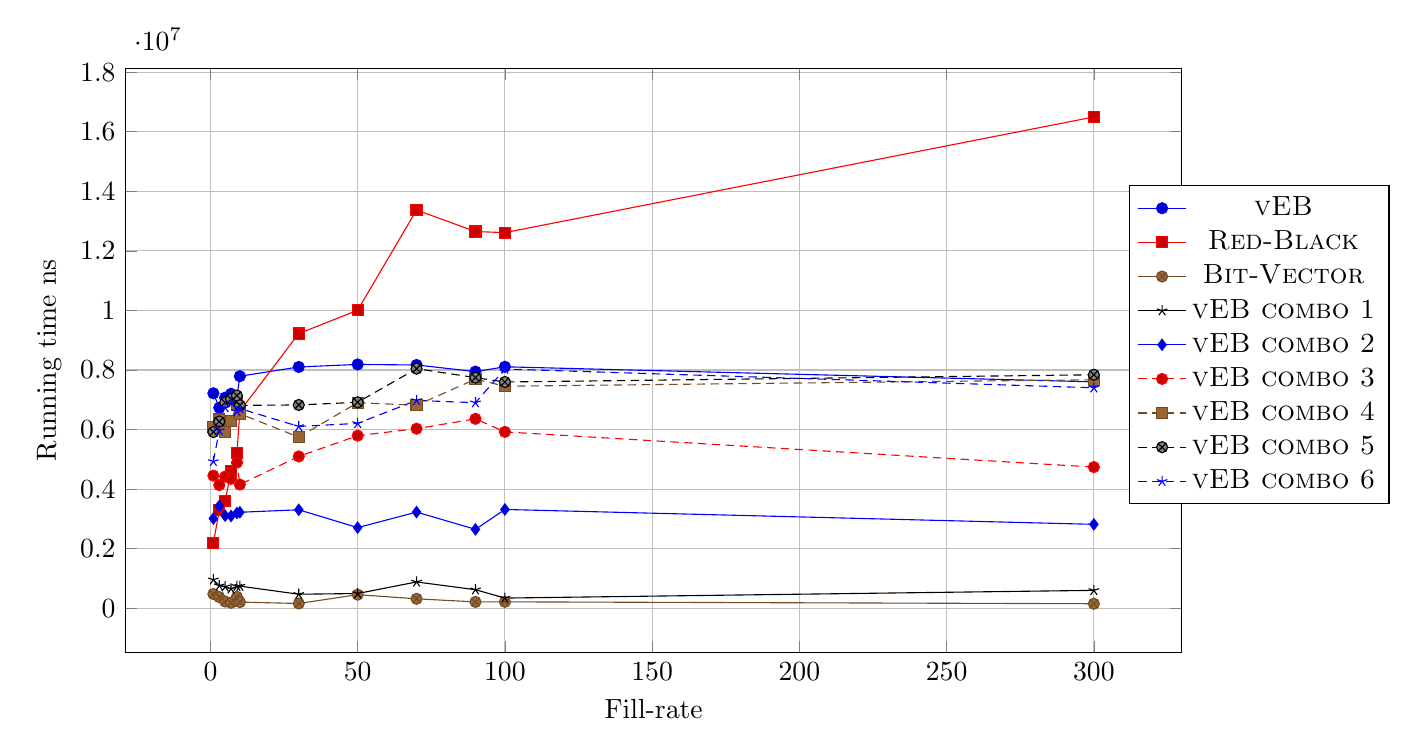
\begin{tikzpicture}
        \begin{axis}[
            xlabel = Fill-rate,
            ylabel = Running time ns,
            height=9cm,
            width=15cm,
            grid=major,
            legend style={
            at={(0.95,0.8)},
            anchor=north west}]            
            legend pos=center west
    	]
    		
    		
    	\addplot coordinates {
(1,7219482)
(3,6732890)
(5,7073095)
(7,7201487)
(9,7099233)
(10,7792185)
(30,8103234)
(50,8187724)
(70,8169491)
(90,7947377)
(100,8108861)
(300,7603375)

    	};
        
    	\addlegendentry{\textsc{vEB}}

                \addplot coordinates {
(1,2191537)
(3,3290645)
(5,3593433)
(7,4614962)
(9,5218118)
(10,6618364)
(30,9224115)
(50,10007101)
(70,13371836)
(90,12650016)
(100,12613658)
(300,16497269)

    	};
        
    	\addlegendentry{\textsc{Red-Black}}

        \addplot coordinates {
(1,480106)
(3,376517)
(5,227959)
(7,185250)
(9,385296)
(10,208760)
(30,162114)
(50,458376)
(70,318658)
(90,214995)
(100,216826)
(300,153726)

    	};
        
    	\addlegendentry{\textsc{Bit-Vector}}

        \addplot coordinates {
(1,958461)
(3,758761)
(5,723510)
(7,653713)
(9,740422)
(10,744510)
(30,472481)
(50,496379)
(70,884876)
(90,624177)
(100,343867)
(300,602609)

    	};
        
    	\addlegendentry{\textsc{vEB combo 1}}

        \addplot coordinates {
(1,3012319)
(3,3436831)
(5,3109156)
(7,3098740)
(9,3198544)
(10,3224827)
(30,3307617)
(50,2708516)
(70,3230914)
(90,2650983)
(100,3318792)
(300,2818899)

    	};
        
    	\addlegendentry{\textsc{vEB combo 2}}

        \addplot coordinates {
(1,4454488)
(3,4136672)
(5,4422337)
(7,4345496)
(9,4890740)
(10,4154957)
(30,5099861)
(50,5797198)
(70,6030496)
(90,6361919)
(100,5923226)
(300,4741674)

    	};
        
    	\addlegendentry{\textsc{vEB combo 3}}
		
        \addplot coordinates {
(1,6093897)
(3,6337560)
(5,5925672)
(7,6292038)
(9,6841126)
(10,6531367)
(30,5748049)
(50,6905038)
(70,6816244)
(90,7693099)
(100,7456329)
(300,7673907)

    	};
        
    	\addlegendentry{\textsc{vEB combo 4}}
		
        \addplot coordinates {
(1,5918180)
(3,6271176)
(5,6908399)
(7,7026304)
(9,7142854)
(10,6813663)
(30,6827262)
(50,6917360)
(70,8045281)
(90,7745485)
(100,7598121)
(300,7840385)

    	};
        
    	\addlegendentry{\textsc{vEB combo 5}}

        \addplot coordinates {
(1,4930966)
(3,5970226)
(5,6738378)
(7,6908254)
(9,6611793)
(10,6705544)
(30,6105720)
(50,6208980)
(70,6978933)
(90,6903084)
(100,8033932)
(300,7403778)

    	};
        
    	\addlegendentry{\textsc{vEB combo 6}}
		
        \end{axis}

    \end{tikzpicture}
    \captionof{figure}{Time of insertion for fill-rates 1 to 300}
    \label{fig:sample_figure}
    
\end{minipage}


The first test is testing inserts, and we can see that Bit-Vector is the fastest. This comes as no surpise since this can be done in constant time. All of the vEB trees insert in time independently of the fill-rate whereas the Red-Black tree takes longer time depending on how many elements that are in the tree.

What is suprising though is that one layer and even two layers of vEB with bit-vectors as leafes performs very well. What is also suprising is that it only takes around 20 promille before the Red-Black tree is slower than all other tested data structures.

\subsection{Results for testing $\Delete$}

Testing $\Delete$ just fills the tree with random numbers from the entire universe and deletes $EPP$ elements. The graph is adjusted to only shwo the fill-rates for 1 to 50, which is no more 5 percent of $2^{24}$ number of elements.

\begin{minipage}[c]{\textwidth}
\advance\leftskip-2.5cm
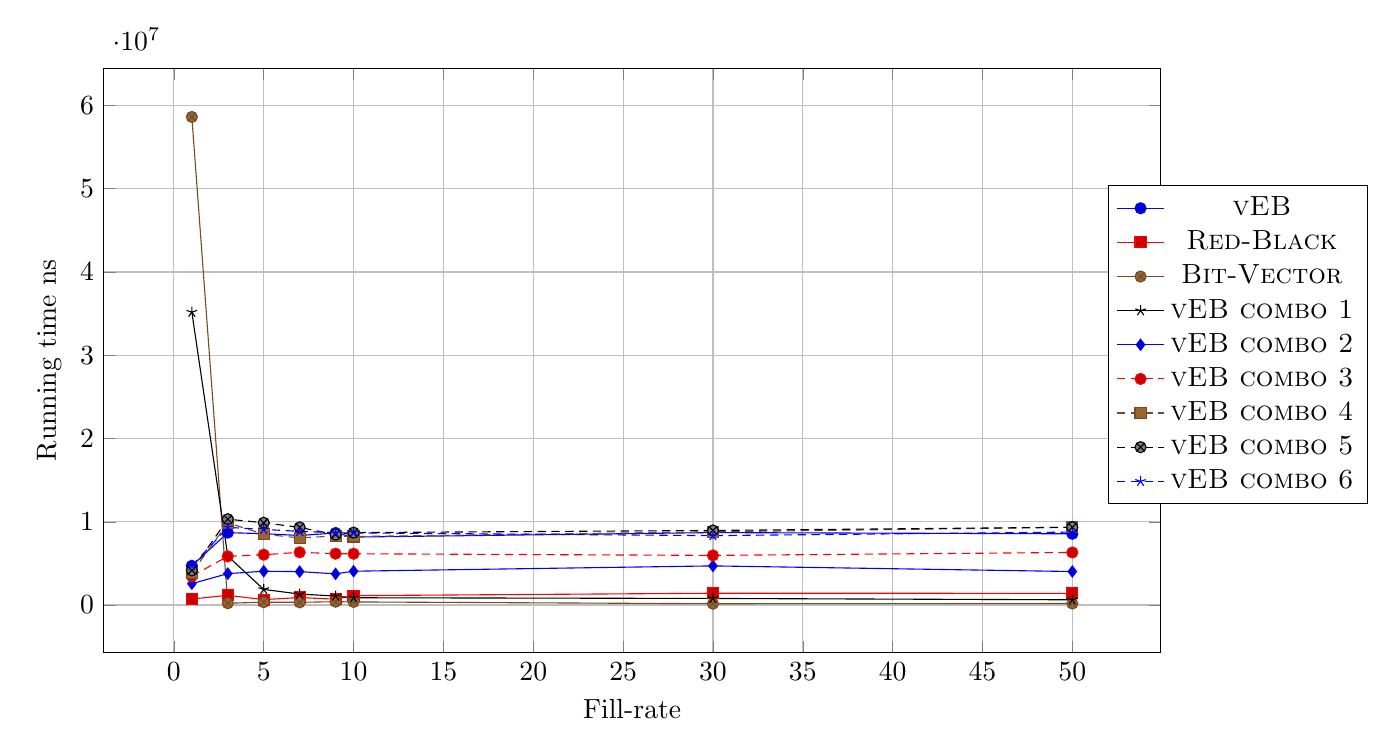
\begin{tikzpicture}
        \begin{axis}[
            xlabel = Fill-rate,
            ylabel = Running time ns,
            height=9cm,
            width=15cm,
            grid=major,
            legend style={
            at={(0.95,0.8)},
            anchor=north west}]            
            legend pos=center west
    	]
    		
    		
    	\addplot coordinates {
(1,4711396)
(3,8698329)
(5,8568622)
(7,8354674)
(9,8653002)
(10,8162417)
(30,8702191)
(50,8556110)

    	};
        
    	\addlegendentry{\textsc{vEB}}

                \addplot coordinates {
(1,723552)
(3,1167318)
(5,655781)
(7,897106)
(9,704127)
(10,1129387)
(30,1418439)
(50,1406950)

    	};
        
    	\addlegendentry{\textsc{Red-Black}}

        \addplot coordinates {
(1,58614407)
(3,217300)
(5,343465)
(7,328333)
(9,403612)
(10,374514)
(30,160266)
(50,181430)

    	};
        
    	\addlegendentry{\textsc{Bit-Vector}}

        \addplot coordinates {
(1,35172148)
(3,5874684)
(5,1876093)
(7,1320925)
(9,1079576)
(10,875917)
(30,792136)
(50,632336)

    	};
        
    	\addlegendentry{\textsc{vEB combo 1}}

        \addplot coordinates {
(1,2565916)
(3,3774592)
(5,4060337)
(7,4014786)
(9,3746261)
(10,4064663)
(30,4701598)
(50,4025325)

    	};
        
    	\addlegendentry{\textsc{vEB combo 2}}

        \addplot coordinates {
(1,3472560)
(3,5843431)
(5,6045389)
(7,6332641)
(9,6166702)
(10,6159200)
(30,5962727)
(50,6314767)

    	};
        
    	\addlegendentry{\textsc{vEB combo 3}}
		
        \addplot coordinates {
(1,3846715)
(3,9872965)
(5,8503351)
(7,8065790)
(9,8297049)
(10,8230956)
(30,8796144)
(50,9337988)

    	};
        
    	\addlegendentry{\textsc{vEB combo 4}}
		
        \addplot coordinates {
(1,4163447)
(3,10311220)
(5,9880559)
(7,9323526)
(9,8461364)
(10,8700218)
(30,8956439)
(50,9342468)

    	};
        
    	\addlegendentry{\textsc{vEB combo 5}}

        \addplot coordinates {
(1,4705049)
(3,9327550)
(5,9085712)
(7,8847626)
(9,8685672)
(10,8663365)
(30,8336582)
(50,8760475)

    	};
        
    	\addlegendentry{\textsc{vEB combo 6}}
		
        \end{axis}

    \end{tikzpicture}
    \captionof{figure}{TITEL}
    \label{fig:sample_figure}
\end{minipage}

It is no suprise that the van Emde Boas Trees are constant with regards to the number of elements in the data structure, however it is suprisingly that $\Delete$ for the Red-Black tree almost is constant too - even for large number of elements. The explanation must be that we are asking to delete elements that exist in the tree such that the amount of misses is kept low and thereby not forcing the algorithm to of $\Delete$ to traverse all the way to the bottom too many times.

$\Delete$ for the Bit-Vector may have to update min or max by using a $\Successor$ or $\Predecessor$ search. However, this is linear worst-case and with a small number of elements in the vector this performs very badly. However, after just 5 promille fill it the most effecient. 

\subsection{Results for testing $\Member$ with guaranteed find}

Testing $\Member$ by filling the tree with random numbers and then takes the first $EPP$ numbers in that sequence and ask for membership. This test is designed so that we are certain the member exists.


\begin{minipage}[c]{\textwidth}
\centering
\begin{tikzpicture}
        \begin{axis}[
            xlabel = \# vertices,
            ylabel = Running time ms,
            height=9cm,
            width=16cm,
            grid=major,
            xtick={0,60000,120000,...,600000},
            scaled x ticks = false,
            legend pos=north west
    	]
    		
    		
    	\addplot coordinates {
(1000,804)
(2000,1640)
(3000,2506)
(4000,3338)
(5000,4220)
(6000,5087)
(7000,5938)
(8000,6776)
(9000,7663)
(10000,8554)
(11000,9435)
(12000,10307)
(13000,11171)
(14000,12028)
(15000,12879)
(16000,13724)
(17000,14608)
(18000,15513)
(19000,16413)
(20000,17307)
(21000,18198)
(22000,19083)
(23000,19965)
(24000,20843)
(25000,21717)
(26000,22588)
(27000,23456)
(28000,24320)
(29000,25181)
(30000,26040)
(31000,26896)
(32000,27749)
(33000,28615)
(34000,29530)
(35000,30442)
(36000,31351)
(37000,32258)
(38000,33162)
(39000,34064)
(40000,34964)
(41000,35862)
(42000,36757)
(43000,37650)
(44000,38542)
(45000,39432)
(46000,40319)
(47000,41205)
(48000,42089)
(49000,42972)
(50000,43852)
(51000,44731)
(52000,45609)
(53000,46485)
(54000,47359)
(55000,48232)
(56000,49104)
(57000,49974)
(58000,50842)
(59000,51710)
(60000,52576)
(61000,53440)
(62000,54304)
(63000,55166)
(64000,56027)
(65000,56887)
(66000,57775)
(67000,58695)
(68000,59613)
(69000,60531)
(70000,61447)
(71000,62361)
(72000,63275)
(73000,64187)
(74000,65099)
(75000,66009)
(76000,66918)
(77000,67826)
(78000,68733)
(79000,69638)
(80000,70543)
(81000,71447)
(82000,72350)
(83000,73251)
(84000,74152)
(85000,75052)
(86000,75951)
(87000,76848)
(88000,77745)
(89000,78642)
(90000,79537)
(91000,80431)
(92000,81324)
(93000,82217)
(94000,83109)
(95000,84000)
(96000,84890)
(97000,85779)
(98000,86667)
(99000,87555)
(100000,88442)
(101000,89328)
(102000,90213)
(103000,91098)
(104000,91982)
(105000,92865)
(106000,93747)
(107000,94629)
(108000,95510)
(109000,96390)
(110000,97269)
(111000,98148)
(112000,99027)
(113000,99904)
(114000,100781)
(115000,101657)
(116000,102533)
(117000,103408)
(118000,104282)
(119000,105156)
(120000,106029)
(121000,106901)
(122000,107773)
(123000,108644)
(124000,109515)
(125000,110385)
(126000,111254)
(127000,112123)
(128000,112991)
(129000,113859)
(130000,114726)
(131000,115593)
(132000,116514)
(133000,117438)
(134000,118361)
(135000,119284)
(136000,120207)
(137000,121129)
(138000,122050)
(139000,122971)
(140000,123891)
(141000,124810)
(142000,125729)
(143000,126647)
(144000,127565)
(145000,128482)
(146000,129399)
(147000,130315)
(148000,131231)
(149000,132146)
(150000,133060)
(151000,133974)
(152000,134888)
(153000,135801)
(154000,136713)
(155000,137625)
(156000,138536)
(157000,139447)
(158000,140358)
(159000,141268)
(160000,142177)
(161000,143086)
(162000,143995)
(163000,144903)
(164000,145810)
(165000,146717)
(166000,147624)
(167000,148530)
(168000,149436)
(169000,150341)
(170000,151246)
(171000,152150)
(172000,153054)
(173000,153957)
(174000,154860)
(175000,155763)
(176000,156665)
(177000,157566)
(178000,158468)
(179000,159369)
(180000,160269)
(181000,161169)
(182000,162069)
(183000,162968)
(184000,163866)
(185000,164765)
(186000,165663)
(187000,166560)
(188000,167457)
(189000,168354)
(190000,169251)
(191000,170147)
(192000,171042)
(193000,171937)
(194000,172832)
(195000,173727)
(196000,174621)
(197000,175514)
(198000,176408)
(199000,177301)
(200000,178193)
(201000,179085)
(202000,179977)
(203000,180869)
(204000,181760)
(205000,182651)
(206000,183541)
(207000,184431)
(208000,185321)
(209000,186210)
(210000,187099)
(211000,187988)
(212000,188876)
(213000,189764)
(214000,190652)
(215000,191539)
(216000,192426)
(217000,193313)
(218000,194199)
(219000,195085)
(220000,195971)
(221000,196856)
(222000,197741)
(223000,198626)
(224000,199510)
(225000,200394)
(226000,201278)
(227000,202161)
(228000,203044)
(229000,203927)
(230000,204809)
(231000,205692)
(232000,206573)
(233000,207455)
(234000,208336)
(235000,209217)
(236000,210098)
(237000,210978)
(238000,211858)
(239000,212738)
(240000,213618)
(241000,214497)
(242000,215376)
(243000,216254)
(244000,217133)
(245000,218011)
(246000,218888)
(247000,219766)
(248000,220643)
(249000,221520)
(250000,222396)
(251000,223273)
(252000,224149)
(253000,225025)
(254000,225900)
(255000,226775)
(256000,227650)
(257000,228525)
(258000,229399)
(259000,230274)
(260000,231148)
(261000,232021)
(262000,232895)
(263000,233815)
(264000,234744)
(265000,235672)
(266000,236600)
(267000,237527)
(268000,238454)
(269000,239381)
(270000,240308)
(271000,241234)
(272000,242160)
(273000,243086)
(274000,244011)
(275000,244937)
(276000,245862)
(277000,246786)
(278000,247711)
(279000,248635)
(280000,249558)
(281000,250482)
(282000,251405)
(283000,252328)
(284000,253251)
(285000,254174)
(286000,255096)
(287000,256018)
(288000,256939)
(289000,257861)
(290000,258782)
(291000,259703)
(292000,260623)
(293000,261544)
(294000,262464)
(295000,263384)
(296000,264303)
(297000,265223)
(298000,266142)
(299000,267061)
(300000,267979)
(301000,268898)
(302000,269816)
(303000,270734)
(304000,271651)
(305000,272569)
(306000,273486)
(307000,274403)
(308000,275319)
(309000,276236)
(310000,277152)
(311000,278068)
(312000,278983)
(313000,279899)
(314000,280814)
(315000,281729)
(316000,282644)
(317000,283558)
(318000,284472)
(319000,285386)
(320000,286300)
(321000,287214)
(322000,288127)
(323000,289040)
(324000,289953)
(325000,290866)
(326000,291778)
(327000,292690)
(328000,293602)
(329000,294514)
(330000,295426)
(331000,296337)
(332000,297248)
(333000,298159)
(334000,299070)
(335000,299980)
(336000,300890)
(337000,301800)
(338000,302710)
(339000,303620)
(340000,304529)
(341000,305438)
(342000,306347)
(343000,307256)
(344000,308165)
(345000,309073)
(346000,309981)
(347000,310889)
(348000,311796)
(349000,312704)
(350000,313611)
(351000,314518)
(352000,315425)
(353000,316332)
(354000,317238)
(355000,318145)
(356000,319051)
(357000,319956)
(358000,320862)
(359000,321768)
(360000,322673)
(361000,323578)
(362000,324483)
(363000,325387)
(364000,326292)
(365000,327196)
(366000,328100)
(367000,329004)
(368000,329908)
(369000,330811)
(370000,331714)
(371000,332618)
(372000,333520)
(373000,334423)
(374000,335326)
(375000,336228)
(376000,337130)
(377000,338032)
(378000,338934)
(379000,339836)
(380000,340737)
(381000,341638)
(382000,342539)
(383000,343440)
(384000,344341)
(385000,345241)
(386000,346141)
(387000,347042)
(388000,347942)
(389000,348841)
(390000,349741)
(391000,350640)
(392000,351539)
(393000,352438)
(394000,353337)
(395000,354236)
(396000,355135)
(397000,356033)
(398000,356931)
(399000,357829)
(400000,358727)
(401000,359624)
(402000,360522)
(403000,361419)
(404000,362316)
(405000,363213)
(406000,364110)
(407000,365007)
(408000,365903)
(409000,366799)
(410000,367695)
(411000,368591)
(412000,369487)
(413000,370383)
(414000,371278)
(415000,372173)
(416000,373068)
(417000,373963)
(418000,374858)
(419000,375753)
(420000,376647)
(421000,377541)
(422000,378435)
(423000,379329)
(424000,380223)
(425000,381117)
(426000,382010)
(427000,382903)
(428000,383796)
(429000,384689)
(430000,385582)
(431000,386475)
(432000,387367)
(433000,388260)
(434000,389152)
(435000,390044)
(436000,390936)
(437000,391827)
(438000,392719)
(439000,393610)
(440000,394502)
(441000,395393)
(442000,396283)
(443000,397174)
(444000,398065)
(445000,398955)
(446000,399846)
(447000,400736)
(448000,401626)
(449000,402516)
(450000,403405)
(451000,404295)
(452000,405184)
(453000,406074)
(454000,406963)
(455000,407852)
(456000,408740)
(457000,409629)
(458000,410517)
(459000,411406)
(460000,412294)
(461000,413182)
(462000,414070)
(463000,414958)
(464000,415845)
(465000,416733)
(466000,417620)
(467000,418507)
(468000,419394)
(469000,420281)
(470000,421168)
(471000,422055)
(472000,422941)
(473000,423828)
(474000,424714)
(475000,425600)
(476000,426486)
(477000,427371)
(478000,428257)
(479000,429143)
(480000,430028)
(481000,430913)
(482000,431798)
(483000,432683)
(484000,433568)
(485000,434453)
(486000,435337)
(487000,436221)
(488000,437106)
(489000,437990)
(490000,438874)
(491000,439758)
(492000,440641)
(493000,441525)
(494000,442408)
(495000,443292)
(496000,444175)
(497000,445058)
(498000,445941)
(499000,446823)
(500000,447706)
(501000,448588)
(502000,449471)
(503000,450353)
(504000,451235)
(505000,452117)
(506000,452999)
(507000,453881)
(508000,454762)
(509000,455644)
(510000,456525)
(511000,457406)
(512000,458287)
(513000,459168)
(514000,460049)
(515000,460930)
(516000,461810)
(517000,462691)
(518000,463571)
(519000,464451)
(520000,465331)
(521000,466211)
(522000,467091)
(523000,467970)
(524000,468850)
(525000,469767)
(526000,470699)
(527000,471631)
(528000,472562)
(529000,473494)
(530000,474425)
(531000,475356)
(532000,476287)
(533000,477218)
(534000,478149)
(535000,479080)
(536000,480010)
(537000,480941)
(538000,481871)
(539000,482801)
(540000,483731)
(541000,484661)
(542000,485590)
(543000,486520)
(544000,487449)
(545000,488379)
(546000,489308)
(547000,490237)
(548000,491166)
(549000,492094)
(550000,493023)
(551000,493952)
(552000,494880)
(553000,495808)
(554000,496736)
(555000,497664)
(556000,498592)
(557000,499520)
(558000,500447)
(559000,501375)
(560000,502302)
(561000,503229)
(562000,504156)
(563000,505083)
(564000,506010)
(565000,506937)
(566000,507863)
(567000,508790)
(568000,509716)
(569000,510642)
(570000,511568)
(571000,512494)
(572000,513420)
(573000,514346)
(574000,515271)
(575000,516197)
(576000,517122)
(577000,518047)
(578000,518972)
(579000,519897)
(580000,520822)
(581000,521746)
(582000,522671)
(583000,523595)
(584000,524520)
(585000,525444)
(586000,526368)
(587000,527292)
(588000,528216)
(589000,529139)
(590000,530063)
(591000,530986)
(592000,531910)
(593000,532833)
(594000,533756)
(595000,534679)
(596000,535602)
(597000,536524)
(598000,537447)
(599000,538369)
(600000,539292)

    	};
        
    	\addlegendentry{\textsc{djk1-bha}}

                \addplot coordinates {
(1000,1556)
(2000,3188)
(3000,4880)
(4000,6508)
(5000,8235)
(6000,9934)
(7000,11601)
(8000,13241)
(9000,14983)
(10000,16730)
(11000,18458)
(12000,20169)
(13000,21865)
(14000,23546)
(15000,25215)
(16000,26873)
(17000,28609)
(18000,30387)
(19000,32155)
(20000,33913)
(21000,35662)
(22000,37403)
(23000,39135)
(24000,40860)
(25000,42578)
(26000,44288)
(27000,45993)
(28000,47691)
(29000,49383)
(30000,51070)
(31000,52751)
(32000,54427)
(33000,56129)
(34000,57929)
(35000,59722)
(36000,61511)
(37000,63295)
(38000,65074)
(39000,66848)
(40000,68618)
(41000,70384)
(42000,72145)
(43000,73903)
(44000,75656)
(45000,77406)
(46000,79152)
(47000,80895)
(48000,82634)
(49000,84369)
(50000,86101)
(51000,87831)
(52000,89557)
(53000,91279)
(54000,92999)
(55000,94716)
(56000,96431)
(57000,98142)
(58000,99851)
(59000,101557)
(60000,103260)
(61000,104961)
(62000,106659)
(63000,108355)
(64000,110049)
(65000,111740)
(66000,113487)
(67000,115298)
(68000,117107)
(69000,118913)
(70000,120717)
(71000,122518)
(72000,124317)
(73000,126114)
(74000,127908)
(75000,129700)
(76000,131490)
(77000,133278)
(78000,135064)
(79000,136847)
(80000,138629)
(81000,140408)
(82000,142186)
(83000,143961)
(84000,145735)
(85000,147507)
(86000,149276)
(87000,151044)
(88000,152811)
(89000,154575)
(90000,156338)
(91000,158098)
(92000,159858)
(93000,161615)
(94000,163371)
(95000,165125)
(96000,166877)
(97000,168628)
(98000,170378)
(99000,172125)
(100000,173872)
(101000,175616)
(102000,177360)
(103000,179101)
(104000,180842)
(105000,182580)
(106000,184318)
(107000,186054)
(108000,187788)
(109000,189521)
(110000,191253)
(111000,192984)
(112000,194713)
(113000,196441)
(114000,198167)
(115000,199892)
(116000,201616)
(117000,203339)
(118000,205060)
(119000,206781)
(120000,208500)
(121000,210217)
(122000,211934)
(123000,213649)
(124000,215364)
(125000,217077)
(126000,218788)
(127000,220499)
(128000,222209)
(129000,223917)
(130000,225625)
(131000,227331)
(132000,229146)
(133000,230967)
(134000,232788)
(135000,234607)
(136000,236425)
(137000,238241)
(138000,240057)
(139000,241872)
(140000,243685)
(141000,245497)
(142000,247308)
(143000,249118)
(144000,250927)
(145000,252735)
(146000,254541)
(147000,256347)
(148000,258151)
(149000,259955)
(150000,261757)
(151000,263558)
(152000,265359)
(153000,267158)
(154000,268956)
(155000,270754)
(156000,272550)
(157000,274345)
(158000,276139)
(159000,277933)
(160000,279725)
(161000,281517)
(162000,283307)
(163000,285097)
(164000,286885)
(165000,288673)
(166000,290460)
(167000,292245)
(168000,294030)
(169000,295814)
(170000,297597)
(171000,299380)
(172000,301161)
(173000,302942)
(174000,304721)
(175000,306500)
(176000,308278)
(177000,310055)
(178000,311831)
(179000,313607)
(180000,315381)
(181000,317155)
(182000,318928)
(183000,320700)
(184000,322471)
(185000,324242)
(186000,326011)
(187000,327780)
(188000,329548)
(189000,331316)
(190000,333082)
(191000,334848)
(192000,336613)
(193000,338377)
(194000,340141)
(195000,341903)
(196000,343665)
(197000,345427)
(198000,347187)
(199000,348947)
(200000,350706)
(201000,352464)
(202000,354222)
(203000,355979)
(204000,357735)
(205000,359491)
(206000,361245)
(207000,363000)
(208000,364753)
(209000,366506)
(210000,368258)
(211000,370009)
(212000,371760)
(213000,373510)
(214000,375259)
(215000,377008)
(216000,378756)
(217000,380503)
(218000,382250)
(219000,383996)
(220000,385741)
(221000,387486)
(222000,389230)
(223000,390974)
(224000,392717)
(225000,394459)
(226000,396201)
(227000,397942)
(228000,399682)
(229000,401422)
(230000,403161)
(231000,404899)
(232000,406637)
(233000,408375)
(234000,410111)
(235000,411848)
(236000,413583)
(237000,415318)
(238000,417052)
(239000,418786)
(240000,420519)
(241000,422252)
(242000,423984)
(243000,425716)
(244000,427447)
(245000,429177)
(246000,430907)
(247000,432636)
(248000,434365)
(249000,436093)
(250000,437820)
(251000,439548)
(252000,441274)
(253000,443000)
(254000,444725)
(255000,446450)
(256000,448175)
(257000,449898)
(258000,451622)
(259000,453344)
(260000,455067)
(261000,456788)
(262000,458510)
(263000,460326)
(264000,462157)
(265000,463987)
(266000,465817)
(267000,467647)
(268000,469476)
(269000,471304)
(270000,473132)
(271000,474959)
(272000,476785)
(273000,478612)
(274000,480437)
(275000,482262)
(276000,484086)
(277000,485910)
(278000,487733)
(279000,489556)
(280000,491378)
(281000,493200)
(282000,495021)
(283000,496842)
(284000,498662)
(285000,500481)
(286000,502301)
(287000,504119)
(288000,505937)
(289000,507754)
(290000,509571)
(291000,511388)
(292000,513204)
(293000,515019)
(294000,516834)
(295000,518648)
(296000,520462)
(297000,522276)
(298000,524089)
(299000,525901)
(300000,527713)
(301000,529524)
(302000,531335)
(303000,533146)
(304000,534956)
(305000,536765)
(306000,538574)
(307000,540382)
(308000,542190)
(309000,543998)
(310000,545805)
(311000,547612)
(312000,549418)
(313000,551223)
(314000,553029)
(315000,554833)
(316000,556638)
(317000,558441)
(318000,560245)
(319000,562048)
(320000,563850)
(321000,565652)
(322000,567453)
(323000,569254)
(324000,571055)
(325000,572855)
(326000,574655)
(327000,576454)
(328000,578253)
(329000,580051)
(330000,581849)
(331000,583647)
(332000,585444)
(333000,587241)
(334000,589037)
(335000,590833)
(336000,592628)
(337000,594423)
(338000,596217)
(339000,598012)
(340000,599805)
(341000,601598)
(342000,603391)
(343000,605184)
(344000,606976)
(345000,608767)
(346000,610558)
(347000,612349)
(348000,614139)
(349000,615929)
(350000,617719)
(351000,619508)
(352000,621297)
(353000,623085)
(354000,624873)
(355000,626660)
(356000,628448)
(357000,630234)
(358000,632021)
(359000,633806)
(360000,635592)
(361000,637377)
(362000,639162)
(363000,640946)
(364000,642730)
(365000,644514)
(366000,646297)
(367000,648080)
(368000,649862)
(369000,651644)
(370000,653426)
(371000,655207)
(372000,656988)
(373000,658769)
(374000,660549)
(375000,662328)
(376000,664108)
(377000,665887)
(378000,667666)
(379000,669444)
(380000,671222)
(381000,672999)
(382000,674777)
(383000,676553)
(384000,678330)
(385000,680106)
(386000,681882)
(387000,683657)
(388000,685432)
(389000,687207)
(390000,688981)
(391000,690755)
(392000,692529)
(393000,694302)
(394000,696075)
(395000,697847)
(396000,699620)
(397000,701391)
(398000,703163)
(399000,704934)
(400000,706705)
(401000,708475)
(402000,710246)
(403000,712015)
(404000,713785)
(405000,715554)
(406000,717323)
(407000,719091)
(408000,720859)
(409000,722627)
(410000,724394)
(411000,726162)
(412000,727928)
(413000,729695)
(414000,731461)
(415000,733227)
(416000,734992)
(417000,736757)
(418000,738522)
(419000,740286)
(420000,742051)
(421000,743814)
(422000,745578)
(423000,747341)
(424000,749104)
(425000,750866)
(426000,752629)
(427000,754390)
(428000,756152)
(429000,757913)
(430000,759674)
(431000,761435)
(432000,763195)
(433000,764955)
(434000,766715)
(435000,768474)
(436000,770233)
(437000,771992)
(438000,773750)
(439000,775509)
(440000,777266)
(441000,779024)
(442000,780781)
(443000,782538)
(444000,784295)
(445000,786051)
(446000,787807)
(447000,789563)
(448000,791318)
(449000,793073)
(450000,794828)
(451000,796583)
(452000,798337)
(453000,800091)
(454000,801844)
(455000,803598)
(456000,805351)
(457000,807103)
(458000,808856)
(459000,810608)
(460000,812360)
(461000,814112)
(462000,815863)
(463000,817614)
(464000,819365)
(465000,821115)
(466000,822865)
(467000,824615)
(468000,826365)
(469000,828114)
(470000,829863)
(471000,831612)
(472000,833360)
(473000,835108)
(474000,836856)
(475000,838604)
(476000,840351)
(477000,842098)
(478000,843845)
(479000,845591)
(480000,847338)
(481000,849083)
(482000,850829)
(483000,852575)
(484000,854320)
(485000,856065)
(486000,857809)
(487000,859553)
(488000,861297)
(489000,863041)
(490000,864785)
(491000,866528)
(492000,868271)
(493000,870014)
(494000,871756)
(495000,873498)
(496000,875240)
(497000,876982)
(498000,878723)
(499000,880464)
(500000,882205)
(501000,883946)
(502000,885686)
(503000,887426)
(504000,889166)
(505000,890905)
(506000,892645)
(507000,894384)
(508000,896122)
(509000,897861)
(510000,899599)
(511000,901337)
(512000,903075)
(513000,904812)
(514000,906550)
(515000,908287)
(516000,910023)
(517000,911760)
(518000,913496)
(519000,915232)
(520000,916968)
(521000,918703)
(522000,920439)
(523000,922174)
(524000,923908)
(525000,925718)
(526000,927558)
(527000,929397)
(528000,931236)
(529000,933074)
(530000,934913)
(531000,936751)
(532000,938589)
(533000,940426)
(534000,942263)
(535000,944100)
(536000,945937)
(537000,947774)
(538000,949610)
(539000,951446)
(540000,953281)
(541000,955117)
(542000,956952)
(543000,958787)
(544000,960621)
(545000,962456)
(546000,964290)
(547000,966124)
(548000,967957)
(549000,969790)
(550000,971623)
(551000,973456)
(552000,975289)
(553000,977121)
(554000,978953)
(555000,980784)
(556000,982616)
(557000,984447)
(558000,986278)
(559000,988109)
(560000,989939)
(561000,991769)
(562000,993599)
(563000,995429)
(564000,997258)
(565000,999088)
(566000,1000916)
(567000,1002745)
(568000,1004573)
(569000,1006402)
(570000,1008230)
(571000,1010057)
(572000,1011885)
(573000,1013712)
(574000,1015539)
(575000,1017365)
(576000,1019192)
(577000,1021018)
(578000,1022844)
(579000,1024669)
(580000,1026495)
(581000,1028320)
(582000,1030145)
(583000,1031970)
(584000,1033794)
(585000,1035618)
(586000,1037442)
(587000,1039266)
(588000,1041089)
(589000,1042913)
(590000,1044736)
(591000,1046559)
(592000,1048381)
(593000,1050203)
(594000,1052025)
(595000,1053847)
(596000,1055669)
(597000,1057490)
(598000,1059311)
(599000,1061132)
(600000,1062953)

    	};
        
    	\addlegendentry{\textsc{djk1-bhp}}

        \addplot coordinates {
(1000,200)
(2000,364)
(3000,519)
(4000,668)
(5000,813)
(6000,956)
(7000,1095)
(8000,1233)
(9000,1370)
(10000,1505)
(11000,1638)
(12000,1771)
(13000,1902)
(14000,2032)
(15000,2162)
(16000,2291)
(17000,2419)
(18000,2546)
(19000,2673)
(20000,2799)
(21000,2925)
(22000,3050)
(23000,3174)
(24000,3298)
(25000,3422)
(26000,3545)
(27000,3668)
(28000,3790)
(29000,3912)
(30000,4034)
(31000,4155)
(32000,4276)
(33000,4396)
(34000,4517)
(35000,4637)
(36000,4756)
(37000,4876)
(38000,4995)
(39000,5114)
(40000,5232)
(41000,5351)
(42000,5469)
(43000,5587)
(44000,5704)
(45000,5822)
(46000,5939)
(47000,6056)
(48000,6173)
(49000,6289)
(50000,6406)
(51000,6522)
(52000,6638)
(53000,6754)
(54000,6869)
(55000,6985)
(56000,7100)
(57000,7215)
(58000,7330)
(59000,7445)
(60000,7560)
(61000,7674)
(62000,7788)
(63000,7903)
(64000,8017)
(65000,8130)
(66000,8244)
(67000,8358)
(68000,8471)
(69000,8585)
(70000,8698)
(71000,8811)
(72000,8924)
(73000,9037)
(74000,9149)
(75000,9262)
(76000,9374)
(77000,9487)
(78000,9599)
(79000,9711)
(80000,9823)
(81000,9935)
(82000,10046)
(83000,10158)
(84000,10270)
(85000,10381)
(86000,10492)
(87000,10604)
(88000,10715)
(89000,10826)
(90000,10937)
(91000,11047)
(92000,11158)
(93000,11269)
(94000,11379)
(95000,11490)
(96000,11600)
(97000,11710)
(98000,11821)
(99000,11931)
(100000,12041)
(101000,12151)
(102000,12260)
(103000,12370)
(104000,12480)
(105000,12589)
(106000,12699)
(107000,12808)
(108000,12918)
(109000,13027)
(110000,13136)
(111000,13245)
(112000,13354)
(113000,13463)
(114000,13572)
(115000,13681)
(116000,13789)
(117000,13898)
(118000,14007)
(119000,14115)
(120000,14224)
(121000,14332)
(122000,14440)
(123000,14549)
(124000,14657)
(125000,14765)
(126000,14873)
(127000,14981)
(128000,15089)
(129000,15196)
(130000,15304)
(131000,15412)
(132000,15520)
(133000,15627)
(134000,15735)
(135000,15842)
(136000,15949)
(137000,16057)
(138000,16164)
(139000,16271)
(140000,16378)
(141000,16486)
(142000,16593)
(143000,16700)
(144000,16806)
(145000,16913)
(146000,17020)
(147000,17127)
(148000,17234)
(149000,17340)
(150000,17447)
(151000,17553)
(152000,17660)
(153000,17766)
(154000,17873)
(155000,17979)
(156000,18085)
(157000,18191)
(158000,18298)
(159000,18404)
(160000,18510)
(161000,18616)
(162000,18722)
(163000,18828)
(164000,18933)
(165000,19039)
(166000,19145)
(167000,19251)
(168000,19356)
(169000,19462)
(170000,19568)
(171000,19673)
(172000,19779)
(173000,19884)
(174000,19989)
(175000,20095)
(176000,20200)
(177000,20305)
(178000,20411)
(179000,20516)
(180000,20621)
(181000,20726)
(182000,20831)
(183000,20936)
(184000,21041)
(185000,21146)
(186000,21251)
(187000,21355)
(188000,21460)
(189000,21565)
(190000,21670)
(191000,21774)
(192000,21879)
(193000,21983)
(194000,22088)
(195000,22192)
(196000,22297)
(197000,22401)
(198000,22506)
(199000,22610)
(200000,22714)
(201000,22819)
(202000,22923)
(203000,23027)
(204000,23131)
(205000,23235)
(206000,23339)
(207000,23443)
(208000,23547)
(209000,23651)
(210000,23755)
(211000,23859)
(212000,23963)
(213000,24067)
(214000,24170)
(215000,24274)
(216000,24378)
(217000,24481)
(218000,24585)
(219000,24689)
(220000,24792)
(221000,24896)
(222000,24999)
(223000,25103)
(224000,25206)
(225000,25309)
(226000,25413)
(227000,25516)
(228000,25619)
(229000,25723)
(230000,25826)
(231000,25929)
(232000,26032)
(233000,26135)
(234000,26238)
(235000,26341)
(236000,26444)
(237000,26547)
(238000,26650)
(239000,26753)
(240000,26856)
(241000,26959)
(242000,27062)
(243000,27165)
(244000,27267)
(245000,27370)
(246000,27473)
(247000,27575)
(248000,27678)
(249000,27781)
(250000,27883)
(251000,27986)
(252000,28088)
(253000,28191)
(254000,28293)
(255000,28396)
(256000,28498)
(257000,28600)
(258000,28703)
(259000,28805)
(260000,28907)
(261000,29010)
(262000,29112)
(263000,29214)
(264000,29316)
(265000,29418)
(266000,29520)
(267000,29623)
(268000,29725)
(269000,29827)
(270000,29929)
(271000,30031)
(272000,30133)
(273000,30234)
(274000,30336)
(275000,30438)
(276000,30540)
(277000,30642)
(278000,30744)
(279000,30845)
(280000,30947)
(281000,31049)
(282000,31150)
(283000,31252)
(284000,31354)
(285000,31455)
(286000,31557)
(287000,31658)
(288000,31760)
(289000,31861)
(290000,31963)
(291000,32064)
(292000,32166)
(293000,32267)
(294000,32369)
(295000,32470)
(296000,32571)
(297000,32673)
(298000,32774)
(299000,32875)
(300000,32976)
(301000,33077)
(302000,33179)
(303000,33280)
(304000,33381)
(305000,33482)
(306000,33583)
(307000,33684)
(308000,33785)
(309000,33886)
(310000,33987)
(311000,34088)
(312000,34189)
(313000,34290)
(314000,34391)
(315000,34492)
(316000,34592)
(317000,34693)
(318000,34794)
(319000,34895)
(320000,34996)
(321000,35096)
(322000,35197)
(323000,35298)
(324000,35398)
(325000,35499)
(326000,35600)
(327000,35700)
(328000,35801)
(329000,35901)
(330000,36002)
(331000,36102)
(332000,36203)
(333000,36303)
(334000,36404)
(335000,36504)
(336000,36605)
(337000,36705)
(338000,36805)
(339000,36906)
(340000,37006)
(341000,37106)
(342000,37206)
(343000,37307)
(344000,37407)
(345000,37507)
(346000,37607)
(347000,37707)
(348000,37808)
(349000,37908)
(350000,38008)
(351000,38108)
(352000,38208)
(353000,38308)
(354000,38408)
(355000,38508)
(356000,38608)
(357000,38708)
(358000,38808)
(359000,38908)
(360000,39008)
(361000,39108)
(362000,39207)
(363000,39307)
(364000,39407)
(365000,39507)
(366000,39607)
(367000,39706)
(368000,39806)
(369000,39906)
(370000,40006)
(371000,40105)
(372000,40205)
(373000,40305)
(374000,40404)
(375000,40504)
(376000,40603)
(377000,40703)
(378000,40802)
(379000,40902)
(380000,41002)
(381000,41101)
(382000,41201)
(383000,41300)
(384000,41399)
(385000,41499)
(386000,41598)
(387000,41698)
(388000,41797)
(389000,41896)
(390000,41996)
(391000,42095)
(392000,42194)
(393000,42294)
(394000,42393)
(395000,42492)
(396000,42591)
(397000,42690)
(398000,42790)
(399000,42889)
(400000,42988)
(401000,43087)
(402000,43186)
(403000,43285)
(404000,43384)
(405000,43483)
(406000,43582)
(407000,43681)
(408000,43780)
(409000,43879)
(410000,43978)
(411000,44077)
(412000,44176)
(413000,44275)
(414000,44374)
(415000,44473)
(416000,44572)
(417000,44671)
(418000,44770)
(419000,44868)
(420000,44967)
(421000,45066)
(422000,45165)
(423000,45264)
(424000,45362)
(425000,45461)
(426000,45560)
(427000,45658)
(428000,45757)
(429000,45856)
(430000,45954)
(431000,46053)
(432000,46152)
(433000,46250)
(434000,46349)
(435000,46447)
(436000,46546)
(437000,46644)
(438000,46743)
(439000,46841)
(440000,46940)
(441000,47038)
(442000,47137)
(443000,47235)
(444000,47334)
(445000,47432)
(446000,47530)
(447000,47629)
(448000,47727)
(449000,47826)
(450000,47924)
(451000,48022)
(452000,48120)
(453000,48219)
(454000,48317)
(455000,48415)
(456000,48514)
(457000,48612)
(458000,48710)
(459000,48808)
(460000,48906)
(461000,49004)
(462000,49103)
(463000,49201)
(464000,49299)
(465000,49397)
(466000,49495)
(467000,49593)
(468000,49691)
(469000,49789)
(470000,49887)
(471000,49985)
(472000,50083)
(473000,50181)
(474000,50279)
(475000,50377)
(476000,50475)
(477000,50573)
(478000,50671)
(479000,50769)
(480000,50867)
(481000,50965)
(482000,51062)
(483000,51160)
(484000,51258)
(485000,51356)
(486000,51454)
(487000,51551)
(488000,51649)
(489000,51747)
(490000,51845)
(491000,51942)
(492000,52040)
(493000,52138)
(494000,52235)
(495000,52333)
(496000,52431)
(497000,52528)
(498000,52626)
(499000,52724)
(500000,52821)
(501000,52919)
(502000,53016)
(503000,53114)
(504000,53212)
(505000,53309)
(506000,53407)
(507000,53504)
(508000,53602)
(509000,53699)
(510000,53797)
(511000,53894)
(512000,53991)
(513000,54089)
(514000,54186)
(515000,54284)
(516000,54381)
(517000,54478)
(518000,54576)
(519000,54673)
(520000,54770)
(521000,54868)
(522000,54965)
(523000,55062)
(524000,55160)
(525000,55257)
(526000,55354)
(527000,55451)
(528000,55549)
(529000,55646)
(530000,55743)
(531000,55840)
(532000,55937)
(533000,56035)
(534000,56132)
(535000,56229)
(536000,56326)
(537000,56423)
(538000,56520)
(539000,56617)
(540000,56714)
(541000,56811)
(542000,56909)
(543000,57006)
(544000,57103)
(545000,57200)
(546000,57297)
(547000,57394)
(548000,57491)
(549000,57588)
(550000,57684)
(551000,57781)
(552000,57878)
(553000,57975)
(554000,58072)
(555000,58169)
(556000,58266)
(557000,58363)
(558000,58460)
(559000,58557)
(560000,58653)
(561000,58750)
(562000,58847)
(563000,58944)
(564000,59041)
(565000,59137)
(566000,59234)
(567000,59331)
(568000,59428)
(569000,59524)
(570000,59621)
(571000,59718)
(572000,59814)
(573000,59911)
(574000,60008)
(575000,60104)
(576000,60201)
(577000,60298)
(578000,60394)
(579000,60491)
(580000,60587)
(581000,60684)
(582000,60781)
(583000,60877)
(584000,60974)
(585000,61070)
(586000,61167)
(587000,61263)
(588000,61360)
(589000,61456)
(590000,61553)
(591000,61649)
(592000,61746)
(593000,61842)
(594000,61939)
(595000,62035)
(596000,62131)
(597000,62228)
(598000,62324)
(599000,62421)
(600000,62517)

    	};
        
    	\addlegendentry{\textsc{djk1-fh1}}

        \addplot coordinates {
(1000,100)
(2000,182)
(3000,259)
(4000,334)
(5000,406)
(6000,478)
(7000,548)
(8000,617)
(9000,685)
(10000,752)
(11000,819)
(12000,885)
(13000,951)
(14000,1016)
(15000,1081)
(16000,1145)
(17000,1209)
(18000,1273)
(19000,1336)
(20000,1399)
(21000,1462)
(22000,1525)
(23000,1587)
(24000,1649)
(25000,1711)
(26000,1772)
(27000,1834)
(28000,1895)
(29000,1956)
(30000,2017)
(31000,2077)
(32000,2138)
(33000,2198)
(34000,2258)
(35000,2318)
(36000,2378)
(37000,2438)
(38000,2497)
(39000,2557)
(40000,2616)
(41000,2675)
(42000,2734)
(43000,2793)
(44000,2852)
(45000,2911)
(46000,2969)
(47000,3028)
(48000,3086)
(49000,3144)
(50000,3203)
(51000,3261)
(52000,3319)
(53000,3377)
(54000,3434)
(55000,3492)
(56000,3550)
(57000,3607)
(58000,3665)
(59000,3722)
(60000,3780)
(61000,3837)
(62000,3894)
(63000,3951)
(64000,4008)
(65000,4065)
(66000,4122)
(67000,4179)
(68000,4235)
(69000,4292)
(70000,4349)
(71000,4405)
(72000,4462)
(73000,4518)
(74000,4574)
(75000,4631)
(76000,4687)
(77000,4743)
(78000,4799)
(79000,4855)
(80000,4911)
(81000,4967)
(82000,5023)
(83000,5079)
(84000,5135)
(85000,5190)
(86000,5246)
(87000,5302)
(88000,5357)
(89000,5413)
(90000,5468)
(91000,5523)
(92000,5579)
(93000,5634)
(94000,5689)
(95000,5745)
(96000,5800)
(97000,5855)
(98000,5910)
(99000,5965)
(100000,6020)
(101000,6075)
(102000,6130)
(103000,6185)
(104000,6240)
(105000,6294)
(106000,6349)
(107000,6404)
(108000,6459)
(109000,6513)
(110000,6568)
(111000,6622)
(112000,6677)
(113000,6731)
(114000,6786)
(115000,6840)
(116000,6895)
(117000,6949)
(118000,7003)
(119000,7057)
(120000,7112)
(121000,7166)
(122000,7220)
(123000,7274)
(124000,7328)
(125000,7382)
(126000,7436)
(127000,7490)
(128000,7544)
(129000,7598)
(130000,7652)
(131000,7706)
(132000,7760)
(133000,7813)
(134000,7867)
(135000,7921)
(136000,7975)
(137000,8028)
(138000,8082)
(139000,8135)
(140000,8189)
(141000,8243)
(142000,8296)
(143000,8350)
(144000,8403)
(145000,8456)
(146000,8510)
(147000,8563)
(148000,8617)
(149000,8670)
(150000,8723)
(151000,8776)
(152000,8830)
(153000,8883)
(154000,8936)
(155000,8989)
(156000,9042)
(157000,9095)
(158000,9149)
(159000,9202)
(160000,9255)
(161000,9308)
(162000,9361)
(163000,9414)
(164000,9466)
(165000,9519)
(166000,9572)
(167000,9625)
(168000,9678)
(169000,9731)
(170000,9784)
(171000,9836)
(172000,9889)
(173000,9942)
(174000,9994)
(175000,10047)
(176000,10100)
(177000,10152)
(178000,10205)
(179000,10258)
(180000,10310)
(181000,10363)
(182000,10415)
(183000,10468)
(184000,10520)
(185000,10573)
(186000,10625)
(187000,10677)
(188000,10730)
(189000,10782)
(190000,10835)
(191000,10887)
(192000,10939)
(193000,10991)
(194000,11044)
(195000,11096)
(196000,11148)
(197000,11200)
(198000,11253)
(199000,11305)
(200000,11357)
(201000,11409)
(202000,11461)
(203000,11513)
(204000,11565)
(205000,11617)
(206000,11669)
(207000,11721)
(208000,11773)
(209000,11825)
(210000,11877)
(211000,11929)
(212000,11981)
(213000,12033)
(214000,12085)
(215000,12137)
(216000,12189)
(217000,12240)
(218000,12292)
(219000,12344)
(220000,12396)
(221000,12448)
(222000,12499)
(223000,12551)
(224000,12603)
(225000,12654)
(226000,12706)
(227000,12758)
(228000,12809)
(229000,12861)
(230000,12913)
(231000,12964)
(232000,13016)
(233000,13067)
(234000,13119)
(235000,13170)
(236000,13222)
(237000,13273)
(238000,13325)
(239000,13376)
(240000,13428)
(241000,13479)
(242000,13531)
(243000,13582)
(244000,13633)
(245000,13685)
(246000,13736)
(247000,13787)
(248000,13839)
(249000,13890)
(250000,13941)
(251000,13993)
(252000,14044)
(253000,14095)
(254000,14146)
(255000,14198)
(256000,14249)
(257000,14300)
(258000,14351)
(259000,14402)
(260000,14453)
(261000,14505)
(262000,14556)
(263000,14607)
(264000,14658)
(265000,14709)
(266000,14760)
(267000,14811)
(268000,14862)
(269000,14913)
(270000,14964)
(271000,15015)
(272000,15066)
(273000,15117)
(274000,15168)
(275000,15219)
(276000,15270)
(277000,15321)
(278000,15372)
(279000,15422)
(280000,15473)
(281000,15524)
(282000,15575)
(283000,15626)
(284000,15677)
(285000,15727)
(286000,15778)
(287000,15829)
(288000,15880)
(289000,15931)
(290000,15981)
(291000,16032)
(292000,16083)
(293000,16133)
(294000,16184)
(295000,16235)
(296000,16285)
(297000,16336)
(298000,16387)
(299000,16437)
(300000,16488)
(301000,16539)
(302000,16589)
(303000,16640)
(304000,16690)
(305000,16741)
(306000,16791)
(307000,16842)
(308000,16892)
(309000,16943)
(310000,16993)
(311000,17044)
(312000,17094)
(313000,17145)
(314000,17195)
(315000,17246)
(316000,17296)
(317000,17346)
(318000,17397)
(319000,17447)
(320000,17498)
(321000,17548)
(322000,17598)
(323000,17649)
(324000,17699)
(325000,17749)
(326000,17800)
(327000,17850)
(328000,17900)
(329000,17950)
(330000,18001)
(331000,18051)
(332000,18101)
(333000,18151)
(334000,18202)
(335000,18252)
(336000,18302)
(337000,18352)
(338000,18402)
(339000,18453)
(340000,18503)
(341000,18553)
(342000,18603)
(343000,18653)
(344000,18703)
(345000,18753)
(346000,18803)
(347000,18854)
(348000,18904)
(349000,18954)
(350000,19004)
(351000,19054)
(352000,19104)
(353000,19154)
(354000,19204)
(355000,19254)
(356000,19304)
(357000,19354)
(358000,19404)
(359000,19454)
(360000,19504)
(361000,19554)
(362000,19603)
(363000,19653)
(364000,19703)
(365000,19753)
(366000,19803)
(367000,19853)
(368000,19903)
(369000,19953)
(370000,20003)
(371000,20052)
(372000,20102)
(373000,20152)
(374000,20202)
(375000,20252)
(376000,20301)
(377000,20351)
(378000,20401)
(379000,20451)
(380000,20501)
(381000,20550)
(382000,20600)
(383000,20650)
(384000,20699)
(385000,20749)
(386000,20799)
(387000,20849)
(388000,20898)
(389000,20948)
(390000,20998)
(391000,21047)
(392000,21097)
(393000,21147)
(394000,21196)
(395000,21246)
(396000,21295)
(397000,21345)
(398000,21395)
(399000,21444)
(400000,21494)
(401000,21543)
(402000,21593)
(403000,21642)
(404000,21692)
(405000,21741)
(406000,21791)
(407000,21841)
(408000,21890)
(409000,21940)
(410000,21989)
(411000,22038)
(412000,22088)
(413000,22137)
(414000,22187)
(415000,22236)
(416000,22286)
(417000,22335)
(418000,22385)
(419000,22434)
(420000,22483)
(421000,22533)
(422000,22582)
(423000,22632)
(424000,22681)
(425000,22730)
(426000,22780)
(427000,22829)
(428000,22878)
(429000,22928)
(430000,22977)
(431000,23026)
(432000,23076)
(433000,23125)
(434000,23174)
(435000,23223)
(436000,23273)
(437000,23322)
(438000,23371)
(439000,23421)
(440000,23470)
(441000,23519)
(442000,23568)
(443000,23617)
(444000,23667)
(445000,23716)
(446000,23765)
(447000,23814)
(448000,23863)
(449000,23913)
(450000,23962)
(451000,24011)
(452000,24060)
(453000,24109)
(454000,24158)
(455000,24207)
(456000,24257)
(457000,24306)
(458000,24355)
(459000,24404)
(460000,24453)
(461000,24502)
(462000,24551)
(463000,24600)
(464000,24649)
(465000,24698)
(466000,24747)
(467000,24796)
(468000,24845)
(469000,24894)
(470000,24943)
(471000,24992)
(472000,25041)
(473000,25090)
(474000,25139)
(475000,25188)
(476000,25237)
(477000,25286)
(478000,25335)
(479000,25384)
(480000,25433)
(481000,25482)
(482000,25531)
(483000,25580)
(484000,25629)
(485000,25678)
(486000,25727)
(487000,25775)
(488000,25824)
(489000,25873)
(490000,25922)
(491000,25971)
(492000,26020)
(493000,26069)
(494000,26118)
(495000,26166)
(496000,26215)
(497000,26264)
(498000,26313)
(499000,26362)
(500000,26410)
(501000,26459)
(502000,26508)
(503000,26557)
(504000,26606)
(505000,26654)
(506000,26703)
(507000,26752)
(508000,26801)
(509000,26849)
(510000,26898)
(511000,26947)
(512000,26995)
(513000,27044)
(514000,27093)
(515000,27142)
(516000,27190)
(517000,27239)
(518000,27288)
(519000,27336)
(520000,27385)
(521000,27434)
(522000,27482)
(523000,27531)
(524000,27580)
(525000,27628)
(526000,27677)
(527000,27725)
(528000,27774)
(529000,27823)
(530000,27871)
(531000,27920)
(532000,27968)
(533000,28017)
(534000,28066)
(535000,28114)
(536000,28163)
(537000,28211)
(538000,28260)
(539000,28308)
(540000,28357)
(541000,28406)
(542000,28454)
(543000,28503)
(544000,28551)
(545000,28600)
(546000,28648)
(547000,28697)
(548000,28745)
(549000,28794)
(550000,28842)
(551000,28890)
(552000,28939)
(553000,28987)
(554000,29036)
(555000,29084)
(556000,29133)
(557000,29181)
(558000,29230)
(559000,29278)
(560000,29326)
(561000,29375)
(562000,29423)
(563000,29472)
(564000,29520)
(565000,29568)
(566000,29617)
(567000,29665)
(568000,29714)
(569000,29762)
(570000,29810)
(571000,29859)
(572000,29907)
(573000,29955)
(574000,30004)
(575000,30052)
(576000,30100)
(577000,30149)
(578000,30197)
(579000,30245)
(580000,30294)
(581000,30342)
(582000,30390)
(583000,30438)
(584000,30487)
(585000,30535)
(586000,30583)
(587000,30631)
(588000,30680)
(589000,30728)
(590000,30776)
(591000,30824)
(592000,30873)
(593000,30921)
(594000,30969)
(595000,31017)
(596000,31066)
(597000,31114)
(598000,31162)
(599000,31210)
(600000,31258)

    	};
        
    	\addlegendentry{\textsc{djk1-fh2}}


        \end{axis}

    \end{tikzpicture}
    \captionof{figure}{TITEL}
    \label{fig:sample_figure}
\end{minipage}

In this test it is very clear that the more levels of van Emde Boas trees the slower the data structure will be performing $\Member$ search. We also see that the van Emde Boas tree implemented from ~\cite{ITA09} increases do not look constant. This is propably due to how the arithmetic calculations are implemented and we will discuss this later in the report.

\subsection{Results for testing $\Member$ with un-guaranteed find}

Almost the same as above but again we have another sequence of random numbers that we search for. In this way the probability of the element existing in the data-structure increases as the fill-rate increases.


\begin{minipage}[c]{\textwidth}
\centering
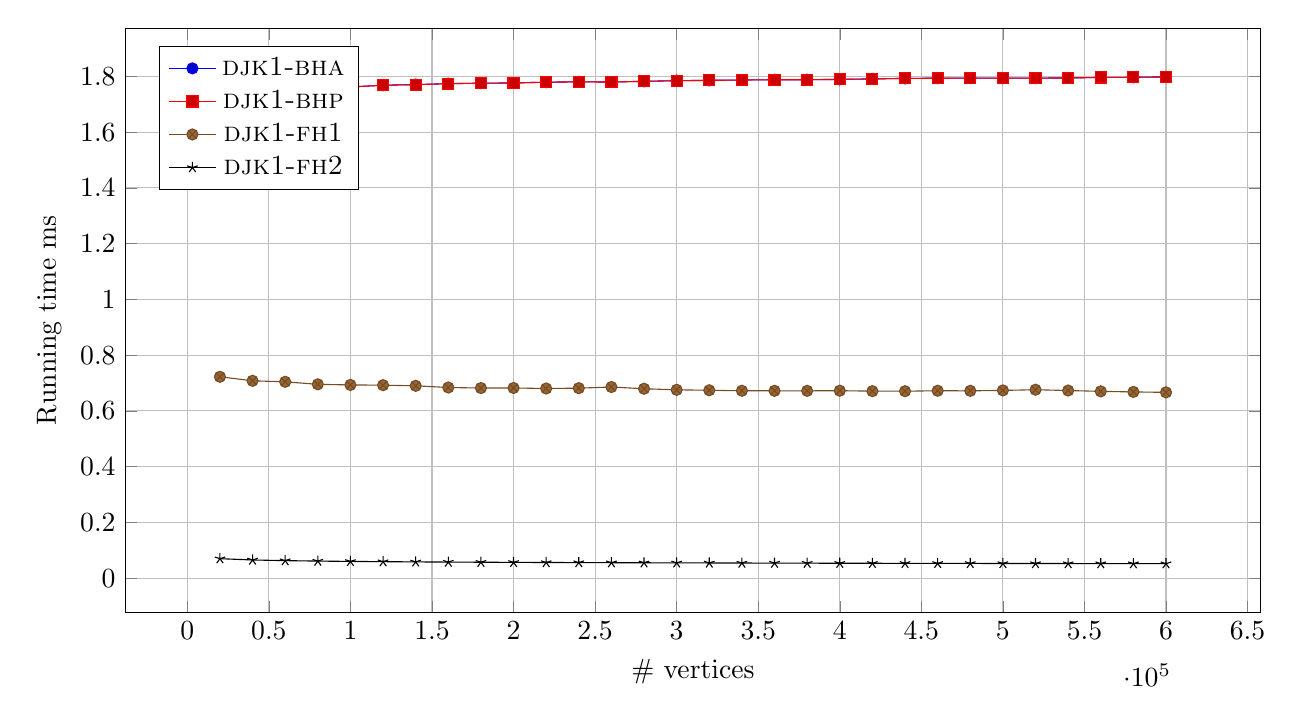
\begin{tikzpicture}
        \begin{axis}[
            xlabel = \# vertices,
            ylabel = Running time ms,
            height=9cm,
            width=16cm,
            grid=major,
            legend pos=north west
    	]
    		
    		
    	\addplot coordinates {
(20000,1.7266)
(40000,1.7463)
(60000,1.7544)
(80000,1.7597)
(100000,1.7621)
(120000,1.7683)
(140000,1.7706)
(160000,1.7740)
(180000,1.7757)
(200000,1.7765)
(220000,1.7793)
(240000,1.7806)
(260000,1.7798)
(280000,1.7824)
(300000,1.7846)
(320000,1.7858)
(340000,1.7871)
(360000,1.7880)
(380000,1.7882)
(400000,1.7893)
(420000,1.7911)
(440000,1.7928)
(460000,1.7935)
(480000,1.7939)
(500000,1.7937)
(520000,1.7938)
(540000,1.7945)
(560000,1.7963)
(580000,1.7969)
(600000,1.7982)

    	};
        
    	\addlegendentry{\textsc{djk1-bha}}

                \addplot coordinates {
(20000,1.7263)
(40000,1.7461)
(60000,1.7543)
(80000,1.7596)
(100000,1.7620)
(120000,1.7683)
(140000,1.7705)
(160000,1.7739)
(180000,1.7756)
(200000,1.7764)
(220000,1.7793)
(240000,1.7805)
(260000,1.7797)
(280000,1.7824)
(300000,1.7845)
(320000,1.7858)
(340000,1.7870)
(360000,1.7879)
(380000,1.7881)
(400000,1.7892)
(420000,1.7910)
(440000,1.7928)
(460000,1.7934)
(480000,1.7938)
(500000,1.7936)
(520000,1.7938)
(540000,1.7944)
(560000,1.7962)
(580000,1.7968)
(600000,1.7982)

    	};
        
    	\addlegendentry{\textsc{djk1-bhp}}

        \addplot coordinates {
(20000,0.7224)
(40000,0.7081)
(60000,0.7045)
(80000,0.6954)
(100000,0.6933)
(120000,0.6924)
(140000,0.6901)
(160000,0.6841)
(180000,0.6821)
(200000,0.6824)
(220000,0.6804)
(240000,0.6817)
(260000,0.6858)
(280000,0.6796)
(300000,0.6757)
(320000,0.6741)
(340000,0.6723)
(360000,0.6722)
(380000,0.6721)
(400000,0.6726)
(420000,0.6710)
(440000,0.6708)
(460000,0.6724)
(480000,0.6721)
(500000,0.6736)
(520000,0.6761)
(540000,0.6732)
(560000,0.6702)
(580000,0.6682)
(600000,0.6666)

    	};
        
    	\addlegendentry{\textsc{djk1-fh1}}

        \addplot coordinates {
(20000,0.0700)
(40000,0.0654)
(60000,0.0630)
(80000,0.0614)
(100000,0.0602)
(120000,0.0593)
(140000,0.0585)
(160000,0.0578)
(180000,0.0573)
(200000,0.0568)
(220000,0.0563)
(240000,0.0560)
(260000,0.0556)
(280000,0.0553)
(300000,0.0550)
(320000,0.0547)
(340000,0.0544)
(360000,0.0542)
(380000,0.0539)
(400000,0.0537)
(420000,0.0535)
(440000,0.0533)
(460000,0.0532)
(480000,0.0530)
(500000,0.0528)
(520000,0.0527)
(540000,0.0525)
(560000,0.0524)
(580000,0.0522)
(600000,0.0521)

    	};
        
    	\addlegendentry{\textsc{djk1-fh2}}


        \end{axis}

    \end{tikzpicture}
    \captionof{figure}{TITEL}
    \label{fig:sample_figure}
\end{minipage}

The results are pretty similar to the results above but but the lines seems more straight. This is probably due to the number of misses is higher such that searching in the interval is more consistent.

\subsection{Results for testing $\Successor$ with guaranteed find}

Testing $\Successor$ by filling the tree with random numbers and then takes the first $EPP$ numbers in that sequence and ask for their successor. This test is designed so that we are certain the successor exists.

\begin{minipage}[c]{\textwidth}
\advance\leftskip-2.5cm
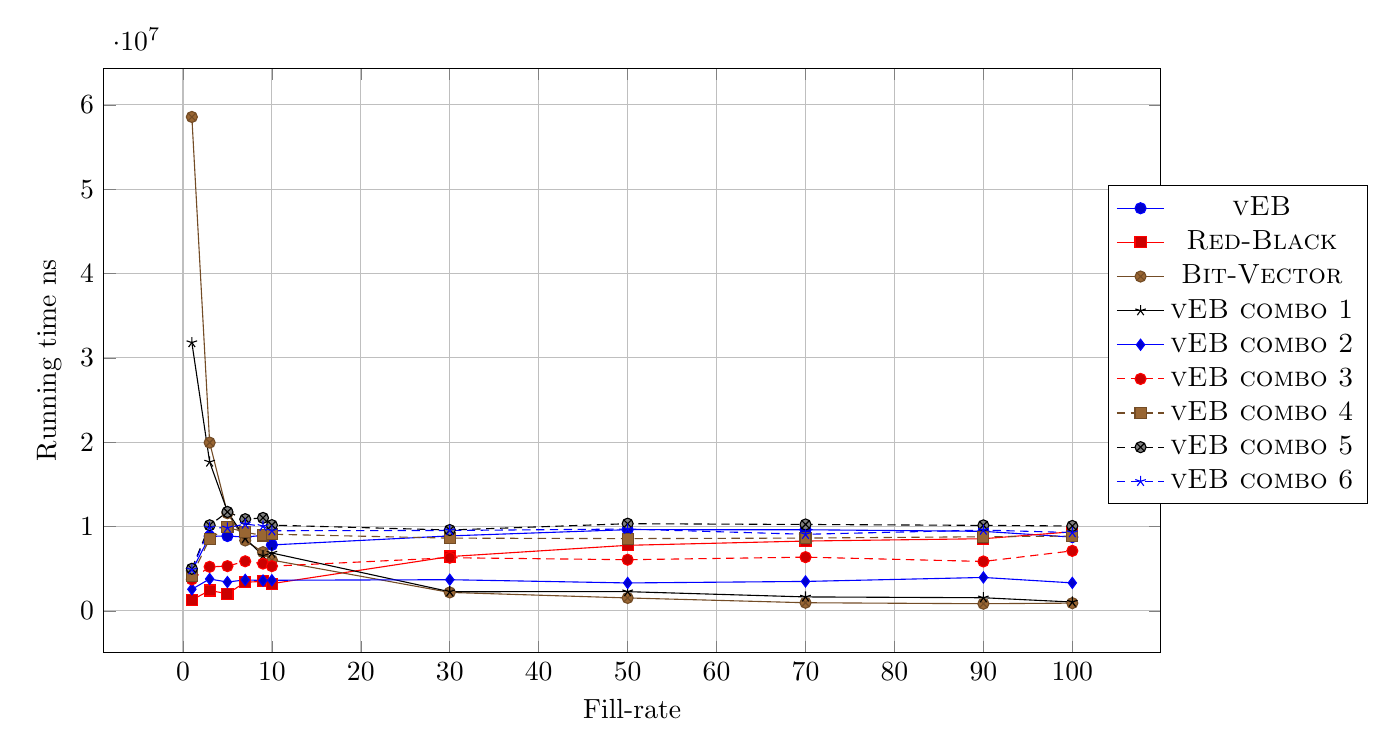
\begin{tikzpicture}
        \begin{axis}[
            xlabel = Fill-rate,
            ylabel = Running time ns,
            height=9cm,
            width=15cm,
            grid=major,
            legend style={
            at={(0.95,0.8)},
            anchor=north west}]            
            legend pos=center west
    	]
    		
    		
    	\addplot coordinates {
(1,4737895)
(3,8839146)
(5,8873758)
(7,8748366)
(9,8952948)
(10,7817276)
(30,8887321)
(50,9627021)
(70,9619006)
(90,9428353)
(100,8745150)

    	};
        
    	\addlegendentry{\textsc{vEB}}

                \addplot coordinates {
(1,1295711)
(3,2414887)
(5,2031312)
(7,3391775)
(9,3494930)
(10,3228139)
(30,6436359)
(50,7771460)
(70,8278056)
(90,8553778)
(100,9377076)

    	};
        
    	\addlegendentry{\textsc{Red-Black}}

        \addplot coordinates {
(1,58566622)
(3,19953045)
(5,11576731)
(7,8343177)
(9,6961951)
(10,6018947)
(30,2185325)
(50,1532243)
(70,962887)
(90,845394)
(100,917697)

    	};
        
    	\addlegendentry{\textsc{Bit-Vector}}

        \addplot coordinates {
(1,31813014)
(3,17655312)
(5,11782795)
(7,8593571)
(9,6541291)
(10,6858544)
(30,2270676)
(50,2276590)
(70,1653624)
(90,1555770)
(100,1047138)

    	};
        
    	\addlegendentry{\textsc{vEB combo 1}}

        \addplot coordinates {
(1,2560919)
(3,3781024)
(5,3416842)
(7,3675054)
(9,3595314)
(10,3630248)
(30,3694120)
(50,3309479)
(70,3489112)
(90,3961093)
(100,3317238)

    	};
        
    	\addlegendentry{\textsc{vEB combo 2}}

        \addplot coordinates {
(1,3730656)
(3,5222154)
(5,5302071)
(7,5877773)
(9,5603918)
(10,5300848)
(30,6301561)
(50,6064338)
(70,6369057)
(90,5857598)
(100,7114013)

    	};
        
    	\addlegendentry{\textsc{vEB combo 3}}
		
        \addplot coordinates {
(1,4161948)
(3,8543267)
(5,9910517)
(7,9314201)
(9,8940642)
(10,9083630)
(30,8624995)
(50,8566298)
(70,8630492)
(90,8787685)
(100,8871690)

    	};
        
    	\addlegendentry{\textsc{vEB combo 4}}
		
        \addplot coordinates {
(1,4990705)
(3,10149026)
(5,11732160)
(7,10871755)
(9,11019960)
(10,10166507)
(30,9585608)
(50,10335347)
(70,10243644)
(90,10136954)
(100,10064463)

    	};
        
    	\addlegendentry{\textsc{vEB combo 5}}

        \addplot coordinates {
(1,4873797)
(3,9851255)
(5,9849445)
(7,10293796)
(9,10036180)
(10,9501118)
(30,9533752)
(50,9700622)
(70,9077753)
(90,9580140)
(100,9282002)

    	};
        
    	\addlegendentry{\textsc{vEB combo 6}}
		
        \end{axis}

    \end{tikzpicture}
    \captionof{figure}{TITEL}
    \label{fig:sample_figure}
\end{minipage}

Here we have adjusted the graph to just show a fill-rate between 1 and 100. It is pretty obvious that the Red-Black Tree will continue to grow and take longer and longer time where the van Emde Boas tree is approaching constant time. The full graph can be found in the appendix.

Again is is facinating that it only takes around 0.5 percent before the Bit-Vector and the van Emde Boas tree with one level has competitative running times.

\subsection{Results for testing $\Successor$ with un-guaranteed find}

Almost the same as above but we then generate another sequence of random numbers that we try to find the successor for. In this way we have no idea how easy it is to find the successor and might resemble a more general use-case.


\begin{minipage}[c]{\textwidth}
\advance\leftskip-2.5cm
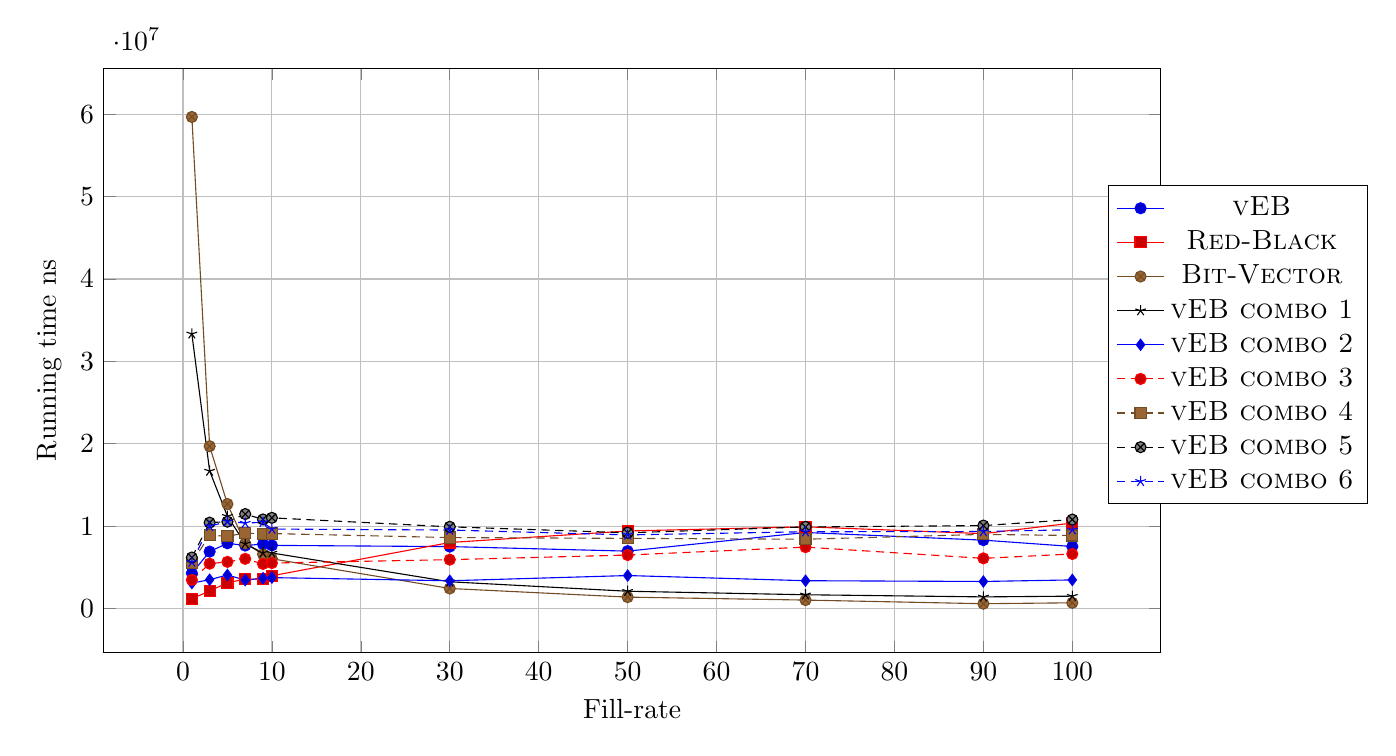
\begin{tikzpicture}
        \begin{axis}[
            xlabel = Fill-rate,
            ylabel = Running time ns,
            height=9cm,
            width=15cm,
            grid=major,
            legend style={
            at={(0.95,0.8)},
            anchor=north west}]            
            legend pos=center west
    	]
    		
    		
    	\addplot coordinates {
(1,4289162)
(3,6904769)
(5,7917724)
(7,7639609)
(9,7822693)
(10,7661854)
(30,7515604)
(50,6964434)
(70,9227038)
(90,8297877)
(100,7525411)

    	};
        
    	\addlegendentry{\textsc{vEB}}

                \addplot coordinates {
(1,1180021)
(3,2136605)
(5,3119509)
(7,3570377)
(9,3579251)
(10,3972629)
(30,8011235)
(50,9410348)
(70,9916202)
(90,9086940)
(100,10371061)

    	};
        
    	\addlegendentry{\textsc{Red-Black}}

        \addplot coordinates {
(1,59661987)
(3,19699905)
(5,12683244)
(7,7889905)
(9,6580509)
(10,6034975)
(30,2431215)
(50,1383201)
(70,1022953)
(90,581727)
(100,693660)

    	};
        
    	\addlegendentry{\textsc{Bit-Vector}}

        \addplot coordinates {
(1,33330593)
(3,16688067)
(5,11203326)
(7,7858158)
(9,6757403)
(10,6738222)
(30,3245082)
(50,2095541)
(70,1668779)
(90,1410375)
(100,1497999)

    	};
        
    	\addlegendentry{\textsc{vEB combo 1}}

        \addplot coordinates {
(1,3084118)
(3,3494945)
(5,4072758)
(7,3443377)
(9,3678475)
(10,3750172)
(30,3366780)
(50,4001223)
(70,3373792)
(90,3281118)
(100,3471132)

    	};
        
    	\addlegendentry{\textsc{vEB combo 2}}

        \addplot coordinates {
(1,3468958)
(3,5443348)
(5,5662853)
(7,6027485)
(9,5409260)
(10,5517193)
(30,5929702)
(50,6489376)
(70,7450711)
(90,6088196)
(100,6619462)

    	};
        
    	\addlegendentry{\textsc{vEB combo 3}}
		
        \addplot coordinates {
(1,5565189)
(3,8890740)
(5,8776827)
(7,9146346)
(9,9074665)
(10,9097010)
(30,8610908)
(50,8512258)
(70,8409364)
(90,8996672)
(100,8861059)

    	};
        
    	\addlegendentry{\textsc{vEB combo 4}}
		
        \addplot coordinates {
(1,6186809)
(3,10424911)
(5,10538703)
(7,11461608)
(9,10811101)
(10,11003884)
(30,9915925)
(50,9191713)
(70,9898874)
(90,10063387)
(100,10794002)

    	};
        
    	\addlegendentry{\textsc{vEB combo 5}}

        \addplot coordinates {
(1,5631937)
(3,9987583)
(5,10558701)
(7,10365672)
(9,10462825)
(10,9643705)
(30,9524555)
(50,8933479)
(70,9315634)
(90,9343570)
(100,9565489)

    	};
        
    	\addlegendentry{\textsc{vEB combo 6}}
		
        \end{axis}

    \end{tikzpicture}
    \captionof{figure}{TITEL}
    \label{fig:sample_figure}
\end{minipage}

Compared to the results before where we had a guaranteed member there is almost no change for the Bit-Vectors and the 1 level van Emde Boas Tree, because the check that the Bit-Vector makes is the same no matter if an element is in the vector or not. 

It is a bit disappointing not seeing a larger change for the Red-Black tree around 100 fill-rate which is about 1.6 million elements.

\subsection{Results for testing $\Minimum$}

Testing $\Minimum$ by calling $\Minimum$ $EPP$ times. The default implementation of a Red-Black Tree do not maintain min and max, so we expect the Red-Black tree to perform much worse than the other data structures when the amount of elements increases.

\begin{minipage}[c]{\textwidth}
\advance\leftskip-2.5cm
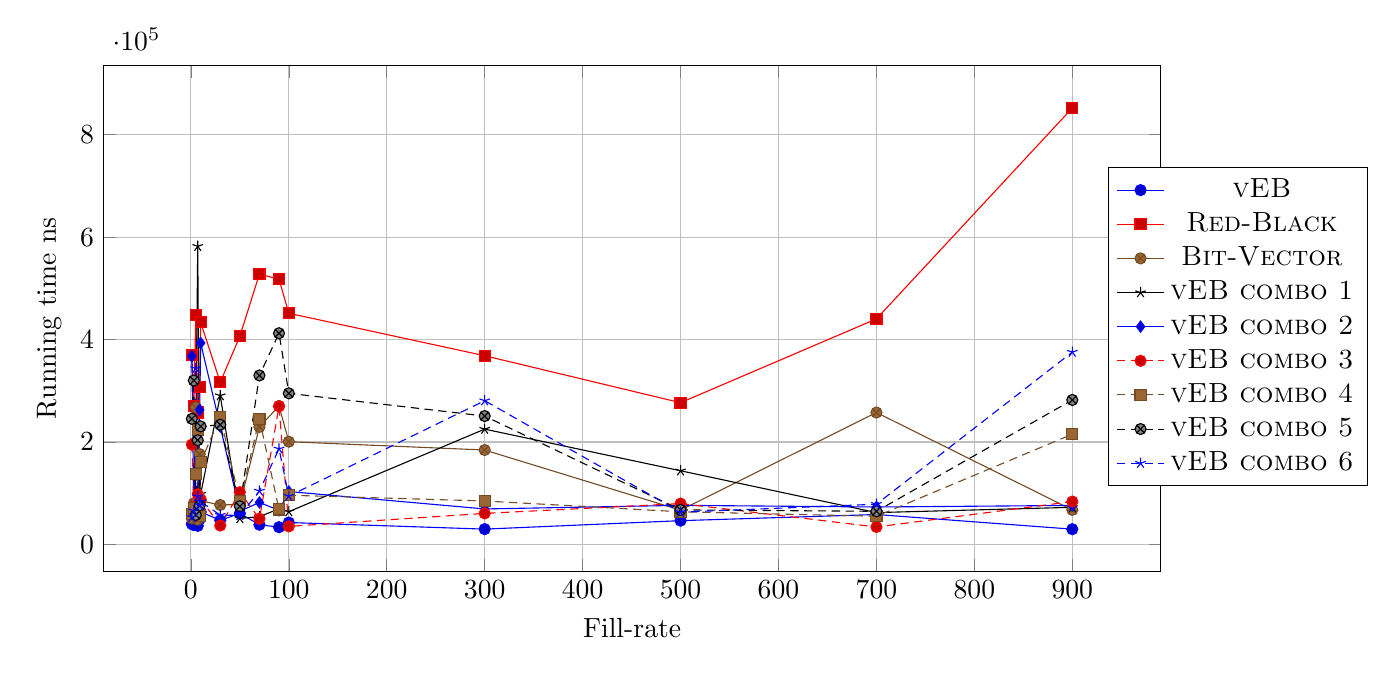
\begin{tikzpicture}
        \begin{axis}[
            xlabel = Fill-rate,
            ylabel = Running time ns,
            height=8cm,
            width=15cm,
            grid=major,
            legend style={
            at={(0.95,0.8)},
            anchor=north west}]            
            legend pos=center west
    	]
    		
    		
    	\addplot coordinates {
(1,39983)
(3,37770)
(5,60090)
(7,36293)
(9,49279)
(10,63464)
(30,47212)
(50,60656)
(70,38569)
(90,33743)
(100,42821)
(300,29939)
(500,46451)
(700,58464)
(900,29848)

    	};
        
    	\addlegendentry{\textsc{vEB}}

                \addplot coordinates {
(1,369656)
(3,269682)
(5,447401)
(7,257775)
(9,306932)
(10,433570)
(30,316599)
(50,406412)
(70,528058)
(90,517502)
(100,451340)
(300,368479)
(500,276750)
(700,440401)
(900,852037)

    	};
        
    	\addlegendentry{\textsc{Red-Black}}

        \addplot coordinates {
(1,50777)
(3,80312)
(5,267680)
(7,48305)
(9,176431)
(10,85122)
(30,77047)
(50,78165)
(70,229418)
(90,270407)
(100,200613)
(300,184392)
(500,66908)
(700,257573)
(900,67491)

    	};
        
    	\addlegendentry{\textsc{Bit-Vector}}

        \addplot coordinates {
(1,66519)
(3,67850)
(5,203066)
(7,582161)
(9,55454)
(10,98147)
(30,290584)
(50,50719)
(70,54353)
(90,69592)
(100,64019)
(300,225163)
(500,143874)
(700,62198)
(900,72529)

    	};
        
    	\addlegendentry{\textsc{vEB combo 1}}

        \addplot coordinates {
(1,367546)
(3,61760)
(5,72775)
(7,79781)
(9,262633)
(10,393288)
(30,230288)
(50,64875)
(70,81913)
(90,66604)
(100,103313)
(300,69349)
(500,76350)
(700,73137)
(900,76164)

    	};
        
    	\addlegendentry{\textsc{vEB combo 2}}

        \addplot coordinates {
(1,194966)
(3,74431)
(5,63885)
(7,97990)
(9,66388)
(10,88192)
(30,36970)
(50,102057)
(70,50254)
(90,269608)
(100,35302)
(300,60655)
(500,79790)
(700,34127)
(900,83763)

    	};
        
    	\addlegendentry{\textsc{vEB combo 3}}
		
        \addplot coordinates {
(1,59287)
(3,70289)
(5,137451)
(7,223670)
(9,55730)
(10,160929)
(30,249064)
(50,84673)
(70,245165)
(90,68293)
(100,96121)
(300,84856)
(500,63808)
(700,55018)
(900,215232)

    	};
        
    	\addlegendentry{\textsc{vEB combo 4}}
		
        \addplot coordinates {
(1,245244)
(3,320063)
(5,57598)
(7,203490)
(9,76171)
(10,230542)
(30,233693)
(50,74470)
(70,329946)
(90,412330)
(100,295031)
(300,250660)
(500,67434)
(700,64749)
(900,282096)

    	};
        
    	\addlegendentry{\textsc{vEB combo 5}}

        \addplot coordinates {
(1,53186)
(3,65756)
(5,343635)
(7,93690)
(9,76575)
(10,83744)
(30,57283)
(50,56702)
(70,104394)
(90,186589)
(100,94347)
(300,280692)
(500,62982)
(700,78576)
(900,375571)

    	};
        
    	\addlegendentry{\textsc{vEB combo 6}}
		
        \end{axis}

    \end{tikzpicture}
    \captionof{figure}{Time of $\Minimum$ search for fill-rates 1 to 900}
    \label{fig:sample_figure}
\end{minipage}


As we can see, the Red-Black tree is slow, even for very small fill-rates. But the results do not entirely match what we anticipated. From fill-rate 100 to 500 the Red-Black Tree actually decreases before it finally rises again. The lowest point in this trendline is actually when the tree is filled with half of the universe.

Every van Emde Boas tree also has something that looks like a similar pattern in the time usage when the tree is half-full. This seems strange since the, however we should note that the difference is around 0.1 of a millisecond.

\section{Summary on search tree results}

The combo tree with two levels of van Emde Boas seems to be the best overall choice considering running time and fill-rates. The bit-vector and the one-layered combo tree suffers from very high query times for successor and predecessor when the fill-rate are below 0.5~0.7 percent which roughly translates to about 100.000 elements, so the combo-tree with two layers looks like a perfect candidate when considering the results of our tests.

\chapter{Testing trees as if they where heaps}

In this chapter we will see how our search trees and Bit-Vector performs compared to our heap implementations from a previous project in the course. We will first briefly describe the priority queues we implemented and their running times, then describe our manufactured tests and finally show how the structures performs on said tests.

\section{Priority Queues from Project 1}

In our last project we implemented four different heaps - A binary heap that used an array as storage, a binary heap that used nodes and pointers and two Fibonacci Heaps.

\begin{center}
  \begin{tabular}{ l | c | c | c }
    Operation & Binary heap & \specialcell{Fibonacci heap v1\\(amortized)} & \specialcell{Fibonacci heap v2\\(amortized)} \\ \hline
    \MakeHeap & $\BigT{1}$ & $\BigT{1}$ & $\BigT{1}$ \\ 
    \FindMin & $\BigT{1}$ & $\BigT{1}$ & $\BigO{l(\log (\frac{n}{l}) + 1)}$\\ 
    \Insert & $\BigT{\log n}$ & $\BigT{1}$ & $\BigT{1}$ \\ 
    \DeleteMin & $\BigT{\log n}$ & $\BigO{\log n}$ & $\BigT{1}$  \\ 
    \DecreaseKey & $\BigT{\log n}$ & $\BigO{1}$ & $\BigO{1}$ \\ 
    \Delete & $\BigT{\log n}$ & $\BigO{\log n}$ & $\BigT{1}$ \\ 
    \Meld & $\BigT{n}$ & $\BigT{1}$ & $\BigT{1}$ \\
  \end{tabular}
\end{center}

\section{Designing tests}

We made a series of tests in the previous project one being inserting a number of elements and deleting them again. The test had the following results:


\begin{minipage}[c]{\textwidth}
\centering
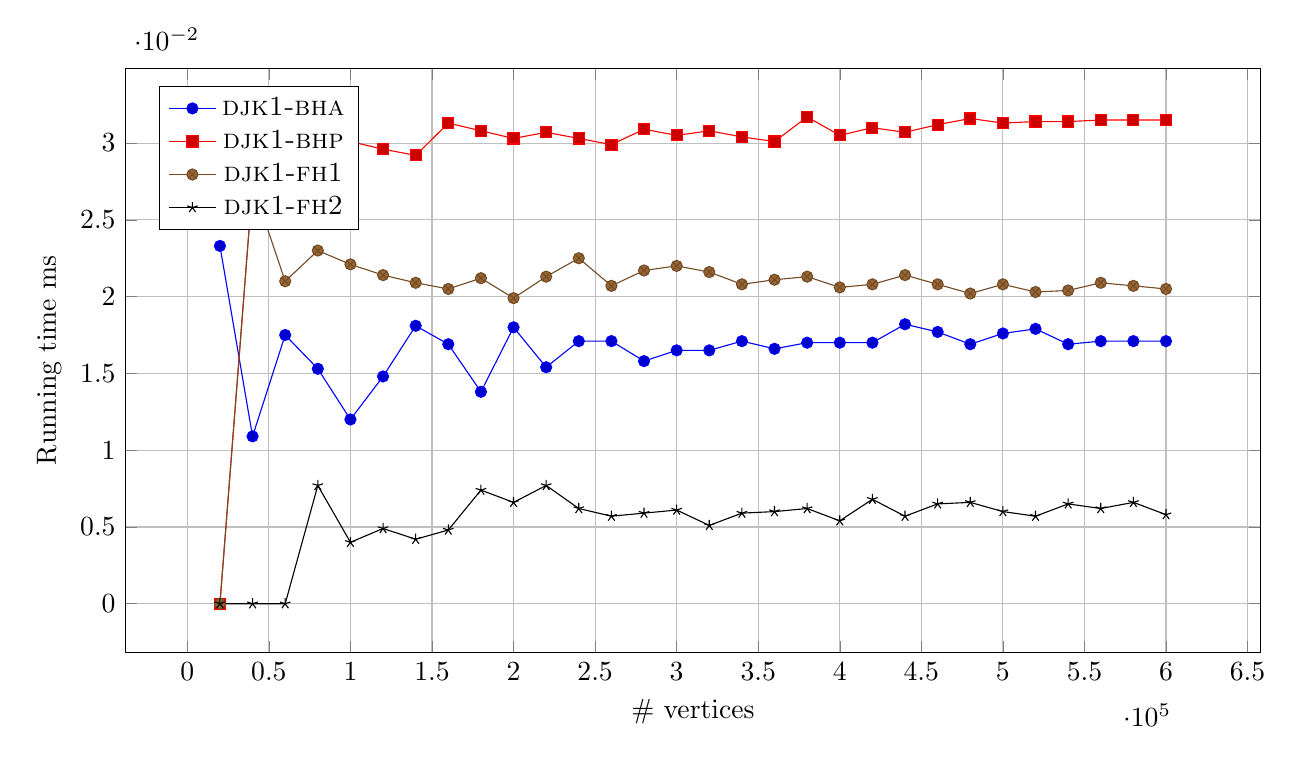
\begin{tikzpicture}
        \begin{axis}[
            xlabel = \# vertices,
            ylabel = Running time ms,
            height=9cm,
            width=16cm,
            grid=major,
            legend pos=north west
    	]
    		
    		
    	\addplot coordinates {
(20000,0.0233)
(40000,0.0109)
(60000,0.0175)
(80000,0.0153)
(100000,0.0120)
(120000,0.0148)
(140000,0.0181)
(160000,0.0169)
(180000,0.0138)
(200000,0.0180)
(220000,0.0154)
(240000,0.0171)
(260000,0.0171)
(280000,0.0158)
(300000,0.0165)
(320000,0.0165)
(340000,0.0171)
(360000,0.0166)
(380000,0.0170)
(400000,0.0170)
(420000,0.0170)
(440000,0.0182)
(460000,0.0177)
(480000,0.0169)
(500000,0.0176)
(520000,0.0179)
(540000,0.0169)
(560000,0.0171)
(580000,0.0171)
(600000,0.0171)

    	};
        
    	\addlegendentry{\textsc{djk1-bha}}

                \addplot coordinates {
(20000,0.0000)
(40000,0.0273)
(60000,0.0280)
(80000,0.0307)
(100000,0.0301)
(120000,0.0296)
(140000,0.0292)
(160000,0.0313)
(180000,0.0308)
(200000,0.0303)
(220000,0.0307)
(240000,0.0303)
(260000,0.0299)
(280000,0.0309)
(300000,0.0305)
(320000,0.0308)
(340000,0.0304)
(360000,0.0301)
(380000,0.0317)
(400000,0.0305)
(420000,0.0310)
(440000,0.0307)
(460000,0.0312)
(480000,0.0316)
(500000,0.0313)
(520000,0.0314)
(540000,0.0314)
(560000,0.0315)
(580000,0.0315)
(600000,0.0315)

    	};
        
    	\addlegendentry{\textsc{djk1-bhp}}

        \addplot coordinates {
(20000,0.0000)
(40000,0.0273)
(60000,0.0210)
(80000,0.0230)
(100000,0.0221)
(120000,0.0214)
(140000,0.0209)
(160000,0.0205)
(180000,0.0212)
(200000,0.0199)
(220000,0.0213)
(240000,0.0225)
(260000,0.0207)
(280000,0.0217)
(300000,0.0220)
(320000,0.0216)
(340000,0.0208)
(360000,0.0211)
(380000,0.0213)
(400000,0.0206)
(420000,0.0208)
(440000,0.0214)
(460000,0.0208)
(480000,0.0202)
(500000,0.0208)
(520000,0.0203)
(540000,0.0204)
(560000,0.0209)
(580000,0.0207)
(600000,0.0205)

    	};
        
    	\addlegendentry{\textsc{djk1-fh1}}

        \addplot coordinates {
(20000,0.0000)
(40000,0.0000)
(60000,0.0000)
(80000,0.0077)
(100000,0.0040)
(120000,0.0049)
(140000,0.0042)
(160000,0.0048)
(180000,0.0074)
(200000,0.0066)
(220000,0.0077)
(240000,0.0062)
(260000,0.0057)
(280000,0.0059)
(300000,0.0061)
(320000,0.0051)
(340000,0.0059)
(360000,0.0060)
(380000,0.0062)
(400000,0.0054)
(420000,0.0068)
(440000,0.0057)
(460000,0.0065)
(480000,0.0066)
(500000,0.0060)
(520000,0.0057)
(540000,0.0065)
(560000,0.0062)
(580000,0.0066)
(600000,0.0058)

    	};
        
    	\addlegendentry{\textsc{djk1-fh2}}


        \end{axis}

    \end{tikzpicture}
    \captionof{figure}{TITEL}
    \label{fig:sample_figure}
\end{minipage}

In general the Fibonacci v2 and Binary Heap with arrays performed the best but as with testing the Red-Black search tree against the van Emde Boas Tree, we have to adjust our test sizes to be expressed in terms of the universe size.

Our search trees do not support the $\DecreaseKey$ operation, so this has been cruedly implemented as a $\Delete$ operation followed by an $\Insert$ operation. Also, we will not test melding or member search since this is not something both types of data structures support.

Another thing to notice is that our heaps require direct indexing for the $\Delete$ operation. For each item we pass to any of the heaps a constant lookup will give the node (position for the array implementation). This can be achievede for the Red-Black tree, which we have done, but not for The van Emde Boas because we only support storing keys from the universe. We do not expect any of the trees to perform better than the heaps for any of the operations besides $\FindMin$ which is a constant operation for all but Fibonacci v2.

Since the Fibonacci heaps have a somewhat lazy approach to when work has to be done, we have decided that we will test the heaps by forcing all remaining work to be completed, which generally amounts to calling $\DeleteMin$ and $\FindMin$. Measering and fill-rates are the same as for testing trees.

\section{Results}

In this section we present the test and the results accompanying them.

\subsection{Results for testing $\Insert$}

 The test for $\Insert$ inserts a certain promille of the entire universe into each data structure followed by a single $\DeleteMin$ and a single $\FindMin$.

\begin{minipage}[c]{\textwidth}
\advance\leftskip-2.5cm
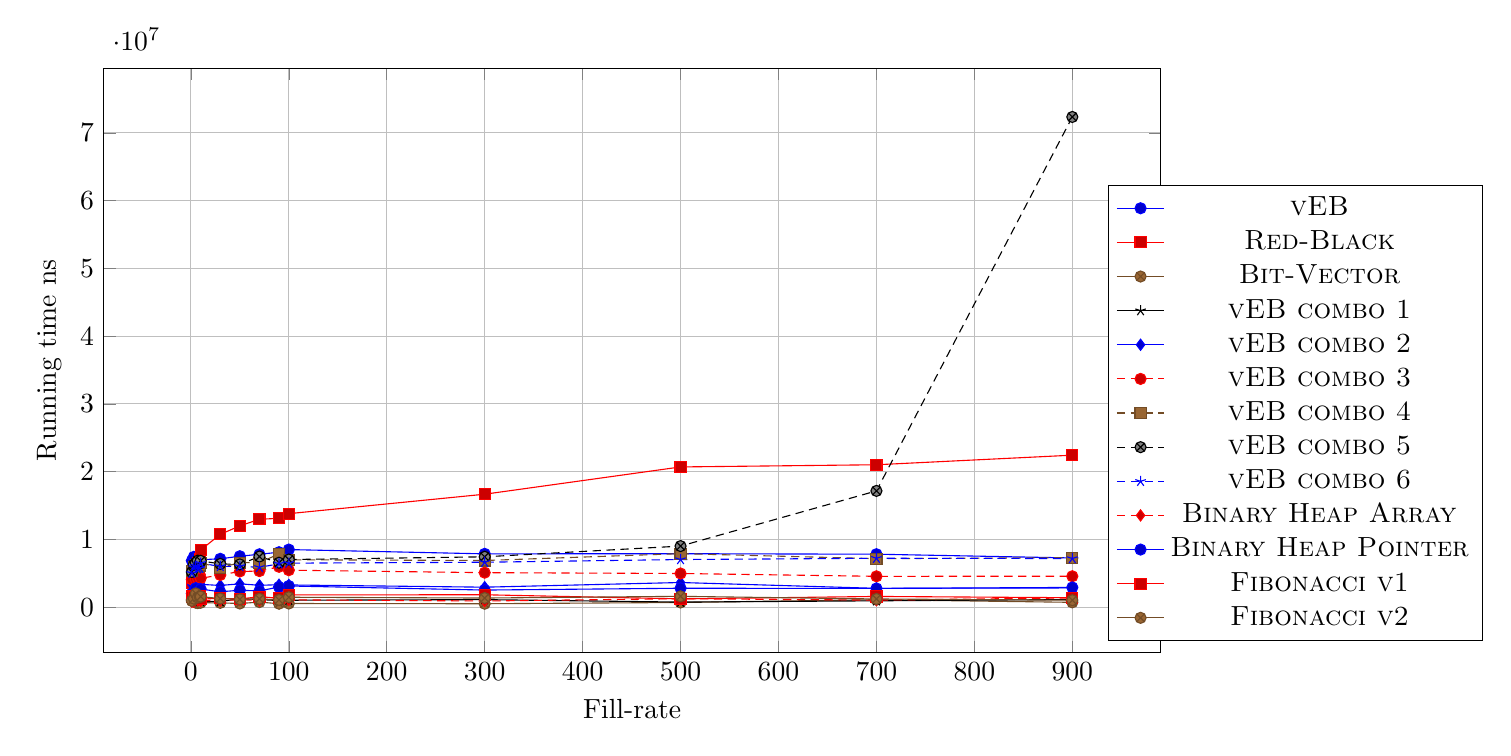
\begin{tikzpicture}
        \begin{axis}[
            xlabel = Fill-rate,
            ylabel = Running time ns,
            height=9cm,
            width=15cm,
            grid=major,
            legend style={
            at={(0.95,0.8)},
            anchor=north west}]            
            legend pos=center west
    	]
    		
    		
    	\addplot coordinates {
(1,6853505)
(3,7423505)
(5,6675328)
(7,7555285)
(9,6658575)
(10,7008460)
(30,7138946)
(50,7520436)
(70,7807058)
(90,8110233)
(100,8502526)
(300,7869190)
(500,7891815)
(700,7818680)
(900,7263690)

    	};
        
    	\addlegendentry{\textsc{vEB}}

                \addplot coordinates {
(1,3594615)
(3,4390370)
(5,5648966)
(7,6470776)
(9,7031702)
(10,8434070)
(30,10742972)
(50,11998132)
(70,12968873)
(90,13116689)
(100,13800857)
(300,16672016)
(500,20696596)
(700,21018861)
(900,22432104)

    	};
        
    	\addlegendentry{\textsc{Red-Black}}

        \addplot coordinates {
(1,1108986)
(3,933524)
(5,661097)
(7,605623)
(9,682659)
(10,654773)
(30,637862)
(50,542250)
(70,751032)
(90,511815)
(100,539724)
(300,508275)
(500,692523)
(700,1106274)
(900,716202)

    	};
        
    	\addlegendentry{\textsc{Bit-Vector}}

        \addplot coordinates {
(1,966015)
(3,896181)
(5,880052)
(7,1398309)
(9,1106360)
(10,870065)
(30,826791)
(50,1263538)
(70,1128709)
(90,975014)
(100,1026700)
(300,1112768)
(500,752027)
(700,940784)
(900,1130809)

    	};
        
    	\addlegendentry{\textsc{vEB combo 1}}

        \addplot coordinates {
(1,3340593)
(3,3430803)
(5,3218563)
(7,3576687)
(9,3116563)
(10,3366387)
(30,3206706)
(50,3447095)
(70,3232419)
(90,3311388)
(100,3280748)
(300,2951999)
(500,3640551)
(700,2781344)
(900,2843018)

    	};
        
    	\addlegendentry{\textsc{vEB combo 2}}

        \addplot coordinates {
(1,4088276)
(3,5119861)
(5,4056704)
(7,4281234)
(9,4806461)
(10,4269001)
(30,4753377)
(50,5269105)
(70,5323451)
(90,5955512)
(100,5457699)
(300,5094679)
(500,4971588)
(700,4554821)
(900,4563138)

    	};
        
    	\addlegendentry{\textsc{vEB combo 3}}
		
        \addplot coordinates {
(1,5388474)
(3,5882206)
(5,6161210)
(7,6010210)
(9,6163718)
(10,6520180)
(30,5843178)
(50,6569060)
(70,6573215)
(90,7853262)
(100,6996064)
(300,6887849)
(500,7904038)
(700,7158620)
(900,7306221)

    	};
        
    	\addlegendentry{\textsc{vEB combo 4}}
		
        \addplot coordinates {
(1,5187723)
(3,6262446)
(5,6541013)
(7,6867455)
(9,6431647)
(10,6842660)
(30,6389414)
(50,6312385)
(70,7474362)
(90,6562913)
(100,7030986)
(300,7432322)
(500,9014987)
(700,17159725)
(900,72344967)

    	};
        
    	\addlegendentry{\textsc{vEB combo 5}}

        \addplot coordinates {
(1,5007968)
(3,5851825)
(5,6068362)
(7,5660941)
(9,5769981)
(10,6495187)
(30,6011735)
(50,6023034)
(70,5883078)
(90,6398691)
(100,6496581)
(300,6633649)
(500,7032237)
(700,7218939)
(900,7182688)

    	};
        
    	\addlegendentry{\textsc{vEB combo 6}}
		
        \addplot coordinates {
(1,787803)
(3,843712)
(5,1251036)
(7,1000649)
(9,1213548)
(10,932348)
(30,967972)
(50,1104452)
(70,999896)
(90,1212147)
(100,1081302)
(300,914446)
(500,1251372)
(700,1040853)
(900,1364707)

    	};
        
    	\addlegendentry{\textsc{Binary Heap Array}}

        \addplot coordinates {
(1,2026234)
(3,2206315)
(5,2811004)
(7,2290128)
(9,2312718)
(10,2671450)
(30,2274271)
(50,2498310)
(70,2398254)
(90,2979110)
(100,3129104)
(300,2527399)
(500,2796667)
(700,2765245)
(900,2915883)

    	};
        
    	\addlegendentry{\textsc{Binary Heap Pointer}}

        \addplot coordinates {
(1,1569308)
(3,1499526)
(5,1587054)
(7,1318099)
(9,1670861)
(10,1196083)
(30,1304231)
(50,1207186)
(70,1554825)
(90,1315199)
(100,1816131)
(300,1832365)
(500,1223560)
(700,1585250)
(900,1396735)

    	};
        
    	\addlegendentry{\textsc{Fibonacci v1}}

        \addplot coordinates {
(1,925469)
(3,1262074)
(5,2033460)
(7,1417833)
(9,1496040)
(10,1566056)
(30,1269833)
(50,1159244)
(70,1234354)
(90,1071215)
(100,1464617)
(300,1350443)
(500,1600869)
(700,1211708)
(900,1024697)

    	};
        
    	\addlegendentry{\textsc{Fibonacci v2}}

        \end{axis}

    \end{tikzpicture}
    \captionof{figure}{Time of $\Insert$ for fill-rates 1 to 900}
    \label{fig:sample_figure}
\end{minipage}


As we can see the Red-Black tree is taking the longest except for one layer of van Emde Boas combined with a bit-vector. The Red-Black tree must wastes some effort being continously balanced so this comes as no surprise, however, it is strange that the one layer of van Emde Boas is performing that bad, but we figure it must be the overhead of bringing such large vectors into memory without giving the computer any possibility of caching. It is a bit hard to see what transpires when the fill-rate is small, so the following figure shows the change from 1 to 50 promille:

\begin{minipage}[c]{\textwidth}
\advance\leftskip-2.5cm
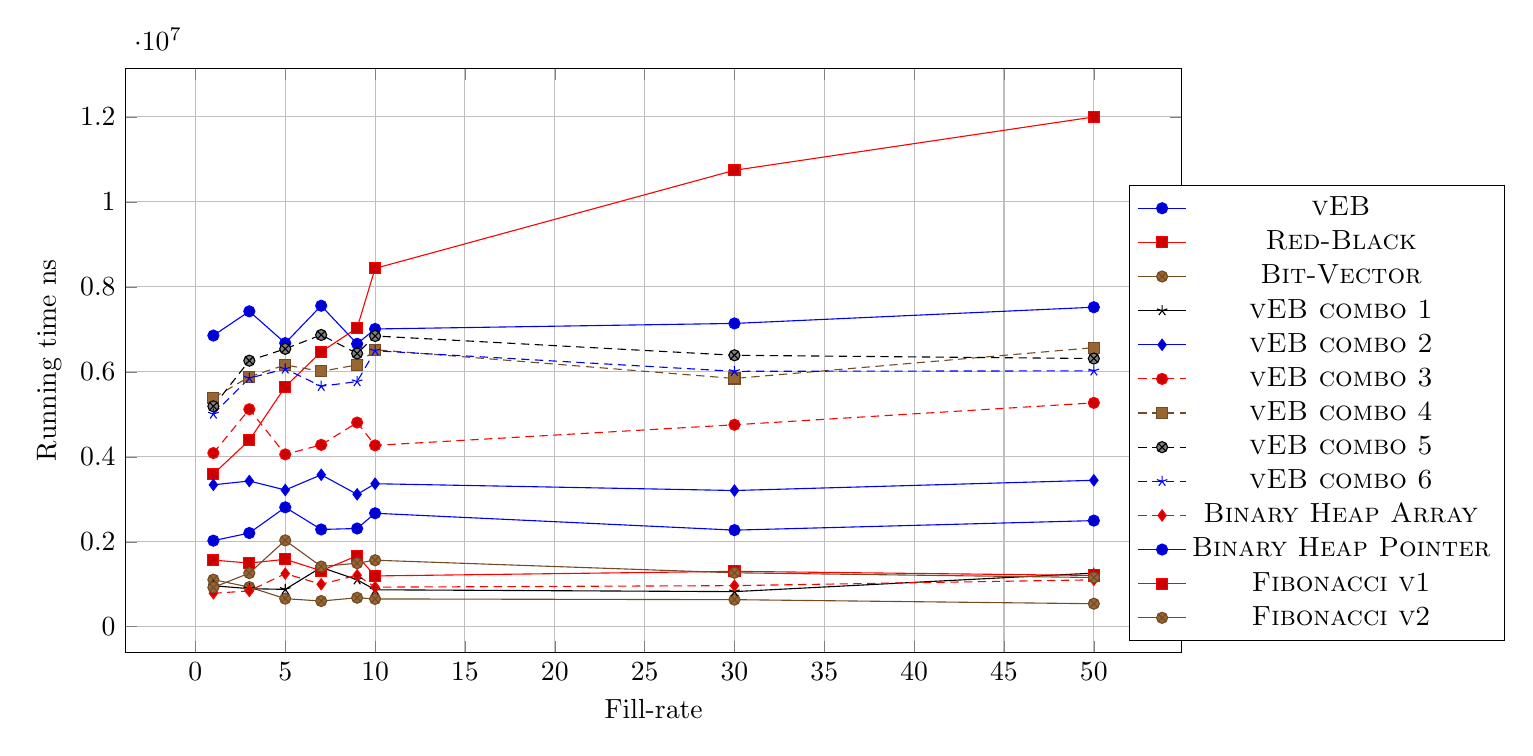
\begin{tikzpicture}
        \begin{axis}[
            xlabel = Fill-rate,
            ylabel = Running time ns,
            height=9cm,
            width=15cm,
            grid=major,
            legend style={
            at={(0.95,0.8)},
            anchor=north west}]            
            legend pos=center west
    	]
    		
    		
    	\addplot coordinates {
(1,6853505)
(3,7423505)
(5,6675328)
(7,7555285)
(9,6658575)
(10,7008460)
(30,7138946)
(50,7520436)

    	};
        
    	\addlegendentry{\textsc{vEB}}

                \addplot coordinates {
(1,3594615)
(3,4390370)
(5,5648966)
(7,6470776)
(9,7031702)
(10,8434070)
(30,10742972)
(50,11998132)

    	};
        
    	\addlegendentry{\textsc{Red-Black}}

        \addplot coordinates {
(1,1108986)
(3,933524)
(5,661097)
(7,605623)
(9,682659)
(10,654773)
(30,637862)
(50,542250)

    	};
        
    	\addlegendentry{\textsc{Bit-Vector}}

        \addplot coordinates {
(1,966015)
(3,896181)
(5,880052)
(7,1398309)
(9,1106360)
(10,870065)
(30,826791)
(50,1263538)

    	};
        
    	\addlegendentry{\textsc{vEB combo 1}}

        \addplot coordinates {
(1,3340593)
(3,3430803)
(5,3218563)
(7,3576687)
(9,3116563)
(10,3366387)
(30,3206706)
(50,3447095)

    	};
        
    	\addlegendentry{\textsc{vEB combo 2}}

        \addplot coordinates {
(1,4088276)
(3,5119861)
(5,4056704)
(7,4281234)
(9,4806461)
(10,4269001)
(30,4753377)
(50,5269105)

    	};
        
    	\addlegendentry{\textsc{vEB combo 3}}
		
        \addplot coordinates {
(1,5388474)
(3,5882206)
(5,6161210)
(7,6010210)
(9,6163718)
(10,6520180)
(30,5843178)
(50,6569060)

    	};
        
    	\addlegendentry{\textsc{vEB combo 4}}
		
        \addplot coordinates {
(1,5187723)
(3,6262446)
(5,6541013)
(7,6867455)
(9,6431647)
(10,6842660)
(30,6389414)
(50,6312385)

    	};
        
    	\addlegendentry{\textsc{vEB combo 5}}

        \addplot coordinates {
(1,5007968)
(3,5851825)
(5,6068362)
(7,5660941)
(9,5769981)
(10,6495187)
(30,6011735)
(50,6023034)

    	};
        
    	\addlegendentry{\textsc{vEB combo 6}}
		
        \addplot coordinates {
(1,787803)
(3,843712)
(5,1251036)
(7,1000649)
(9,1213548)
(10,932348)
(30,967972)
(50,1104452)

    	};
        
    	\addlegendentry{\textsc{Binary Heap Array}}

        \addplot coordinates {
(1,2026234)
(3,2206315)
(5,2811004)
(7,2290128)
(9,2312718)
(10,2671450)
(30,2274271)
(50,2498310)

    	};
        
    	\addlegendentry{\textsc{Binary Heap Pointer}}

        \addplot coordinates {
(1,1569308)
(3,1499526)
(5,1587054)
(7,1318099)
(9,1670861)
(10,1196083)
(30,1304231)
(50,1207186)

    	};
        
    	\addlegendentry{\textsc{Fibonacci v1}}

        \addplot coordinates {
(1,925469)
(3,1262074)
(5,2033460)
(7,1417833)
(9,1496040)
(10,1566056)
(30,1269833)
(50,1159244)

    	};
        
    	\addlegendentry{\textsc{Fibonacci v2}}

        \end{axis}

    \end{tikzpicture}
    \captionof{figure}{TITEL}
    \label{fig:sample_figure}
\end{minipage}

Here we can cleary see that the heaps do perform the best, only interupted by the Bit-Vector which ofcourse has extremely fast inserts. A bit suprising is it to see that van Emde Boas Combo 2, that has two layers, almost matches the binary heap with pointers.

\subsection{Results for testing $\Delete$}

In this test we fill the data-structures with elements and then remove one promille (~16.777) from the data-structure. The deleted keys are guaranteed to be in the structure since our heaps require an existing item to use for deletion. The most action happens inside 50 EPP:

\begin{minipage}[c]{\textwidth}
\advance\leftskip-2.5cm
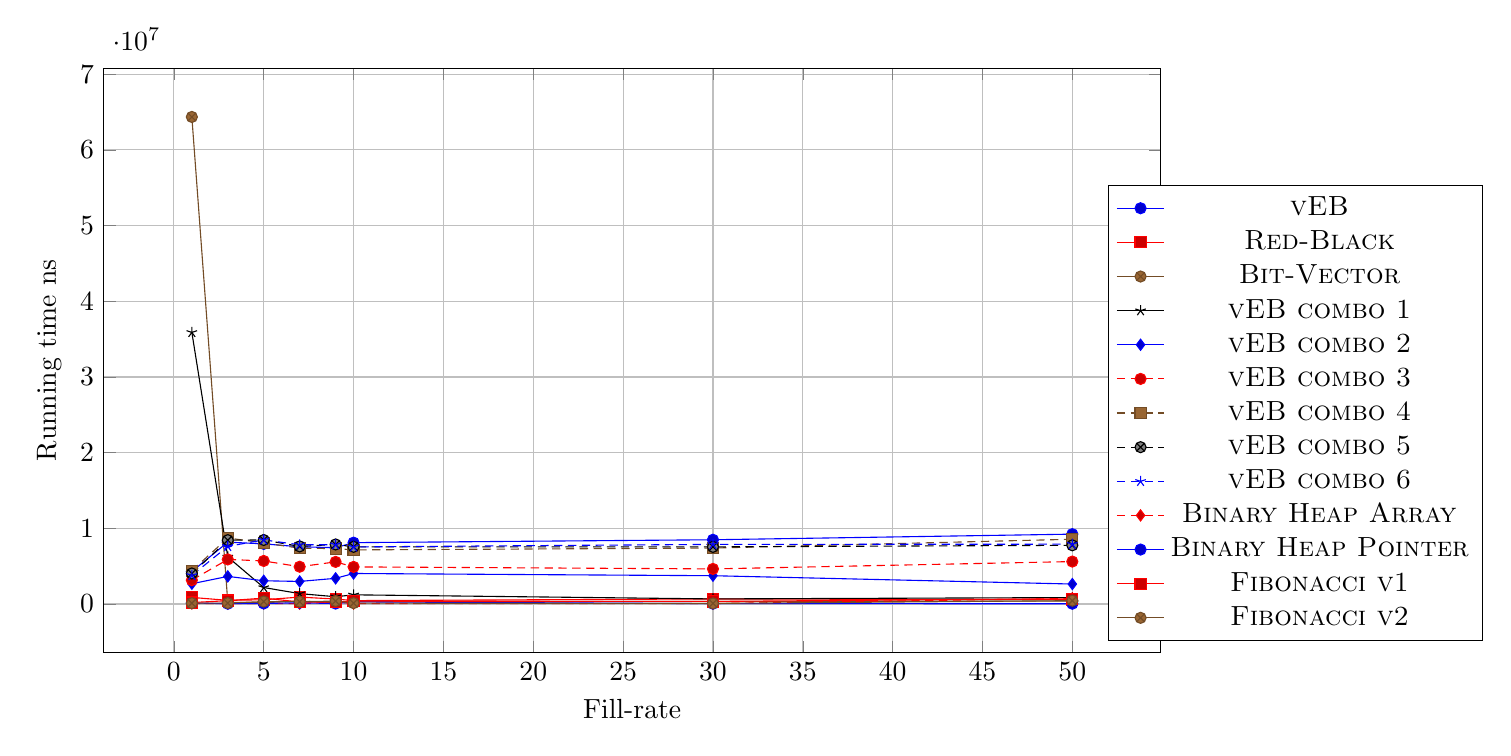
\begin{tikzpicture}
        \begin{axis}[
            xlabel = Fill-rate,
            ylabel = Running time ns,
            height=9cm,
            width=15cm,
            grid=major,
            legend style={
            at={(0.95,0.8)},
            anchor=north west}]            
            legend pos=center west
    	]
    		
    		
    	\addplot coordinates {
(1,4284955)
(3,8175105)
(5,7943693)
(7,7560423)
(9,7440170)
(10,8105875)
(30,8487771)
(50,9228929)

    	};
        
    	\addlegendentry{\textsc{vEB}}

                \addplot coordinates {
(1,867252)
(3,481807)
(5,560854)
(7,911713)
(9,652906)
(10,446657)
(30,668360)
(50,562043)

    	};
        
    	\addlegendentry{\textsc{Red-Black}}

        \addplot coordinates {
(1,64358793)
(3,230533)
(5,175521)
(7,383325)
(9,178819)
(10,325330)
(30,329921)
(50,385495)

    	};
        
    	\addlegendentry{\textsc{Bit-Vector}}

        \addplot coordinates {
(1,35890954)
(3,6213033)
(5,2174950)
(7,1373177)
(9,959584)
(10,1210663)
(30,670256)
(50,847479)

    	};
        
    	\addlegendentry{\textsc{vEB combo 1}}

        \addplot coordinates {
(1,2675300)
(3,3646779)
(5,3068931)
(7,2981376)
(9,3392392)
(10,4030063)
(30,3736876)
(50,2637718)

    	};
        
    	\addlegendentry{\textsc{vEB combo 2}}

        \addplot coordinates {
(1,3150856)
(3,5891374)
(5,5687329)
(7,4923472)
(9,5563293)
(10,4902729)
(30,4636944)
(50,5606111)

    	};
        
    	\addlegendentry{\textsc{vEB combo 3}}
		
        \addplot coordinates {
(1,4404069)
(3,8717274)
(5,8083064)
(7,7369706)
(9,7323853)
(10,7148460)
(30,7392127)
(50,8555472)

    	};
        
    	\addlegendentry{\textsc{vEB combo 4}}
		
        \addplot coordinates {
(1,4032122)
(3,8431899)
(5,8459966)
(7,7610405)
(9,7870767)
(10,7553570)
(30,7548876)
(50,7754571)

    	};
        
    	\addlegendentry{\textsc{vEB combo 5}}

        \addplot coordinates {
(1,3777404)
(3,7613634)
(5,8469041)
(7,7822700)
(9,7831697)
(10,7543435)
(30,7876459)
(50,7904371)

    	};
        
    	\addlegendentry{\textsc{vEB combo 6}}
		
        \addplot coordinates {
(1,75970)
(3,54379)
(5,70125)
(7,48533)
(9,234497)
(10,60380)
(30,57048)
(50,733771)

    	};
        
    	\addlegendentry{\textsc{Binary Heap Array}}

        \addplot coordinates {
(1,140111)
(3,36223)
(5,68472)
(7,162746)
(9,55331)
(10,285601)
(30,43990)
(50,35774)

    	};
        
    	\addlegendentry{\textsc{Binary Heap Pointer}}

        \addplot coordinates {
(1,191504)
(3,440357)
(5,774030)
(7,264811)
(9,237566)
(10,373342)
(30,338775)
(50,693618)

    	};
        
    	\addlegendentry{\textsc{Fibonacci v1}}

        \addplot coordinates {
(1,109756)
(3,119643)
(5,325379)
(7,300177)
(9,384033)
(10,110823)
(30,77872)
(50,438887)

    	};
        
    	\addlegendentry{\textsc{Fibonacci v2}}

        \end{axis}

    \end{tikzpicture}
    \captionof{figure}{TITEL}
    \label{fig:sample_figure}
\end{minipage}

As before in the previous tests the Bit-Vector and one layer performs bad for small fill-rates because that requires to search longer in the array for a minimum and a maximum if one is to be delete.

We see the four heaps performing the best but again followed by the two-layered van Emde Boas Tree, especially for large fill-rates.

\subsection{Results for testing $\DeleteMin$}

In this test we fill the data-structures with elements and the deletes the minimum element EPP times.

\begin{minipage}[c]{\textwidth}
\advance\leftskip-2.5cm
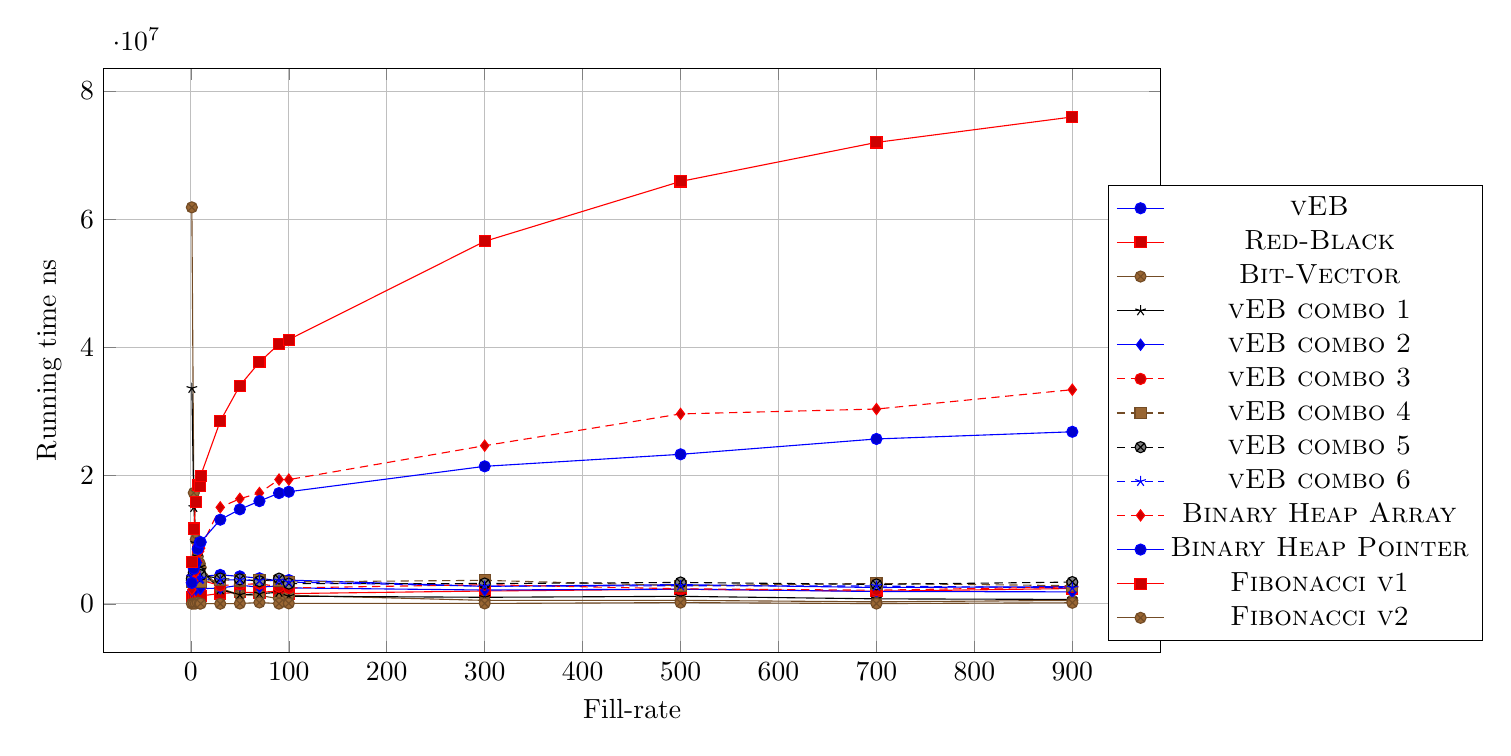
\begin{tikzpicture}
        \begin{axis}[
            xlabel = Fill-rate,
            ylabel = Running time ns,
            height=9cm,
            width=15cm,
            grid=major,
            legend style={
            at={(0.95,0.8)},
            anchor=north west}]            
            legend pos=center west
    	]
    		
    		
    	\addplot coordinates {
(1,3648379)
(3,4609864)
(5,4306113)
(7,4330986)
(9,4302916)
(10,4318578)
(30,4527828)
(50,4306410)
(70,4002612)
(90,3624071)
(100,3722594)
(300,2745651)
(500,3013605)
(700,2562261)
(900,2701766)

    	};
        
    	\addlegendentry{\textsc{vEB}}

                \addplot coordinates {
(1,1002769)
(3,1158938)
(5,1185823)
(7,1578923)
(9,1556382)
(10,1250243)
(30,1635025)
(50,1808039)
(70,1793567)
(90,2022650)
(100,1613647)
(300,2019102)
(500,2294020)
(700,1978919)
(900,2407810)

    	};
        
    	\addlegendentry{\textsc{Red-Black}}

        \addplot coordinates {
(1,61862826)
(3,17325757)
(5,10059959)
(7,7380275)
(9,6327534)
(10,5688375)
(30,2417345)
(50,1451282)
(70,1325879)
(90,810887)
(100,1352968)
(300,556845)
(500,560530)
(700,326917)
(900,551888)

    	};
        
    	\addlegendentry{\textsc{Bit-Vector}}

        \addplot coordinates {
(1,33642289)
(3,15078582)
(5,9470606)
(7,7401396)
(9,5728403)
(10,5293373)
(30,2233118)
(50,1420000)
(70,1587712)
(90,1827105)
(100,1209149)
(300,1038820)
(500,1188997)
(700,793923)
(900,706583)

    	};
        
    	\addlegendentry{\textsc{vEB combo 1}}

        \addplot coordinates {
(1,2082359)
(3,2617851)
(5,2249978)
(7,2969452)
(9,2434432)
(10,2385945)
(30,2467503)
(50,2928565)
(70,2601731)
(90,2833707)
(100,2500337)
(300,2171158)
(500,2314308)
(700,1940326)
(900,1886491)

    	};
        
    	\addlegendentry{\textsc{vEB combo 2}}

        \addplot coordinates {
(1,3351081)
(3,4640796)
(5,3755365)
(7,3892993)
(9,3533979)
(10,3715206)
(30,2870956)
(50,3048141)
(70,3147753)
(90,2682897)
(100,2497146)
(300,3007190)
(500,2362620)
(700,2143535)
(900,2659265)

    	};
        
    	\addlegendentry{\textsc{vEB combo 3}}
		
        \addplot coordinates {
(1,3501897)
(3,4929158)
(5,4659257)
(7,4303371)
(9,4009084)
(10,3470820)
(30,3744964)
(50,3664352)
(70,3729518)
(90,3566699)
(100,3438581)
(300,3682307)
(500,2845434)
(700,3198165)
(900,2848460)

    	};
        
    	\addlegendentry{\textsc{vEB combo 4}}
		
        \addplot coordinates {
(1,3947440)
(3,4902814)
(5,4993596)
(7,4284642)
(9,4915518)
(10,4492834)
(30,3957196)
(50,3833291)
(70,3551924)
(90,3954975)
(100,3170624)
(300,3182026)
(500,3352146)
(700,3051133)
(900,3410003)

    	};
        
    	\addlegendentry{\textsc{vEB combo 5}}

        \addplot coordinates {
(1,4232740)
(3,4323363)
(5,4765986)
(7,4091007)
(9,3860862)
(10,3930572)
(30,3747057)
(50,3747800)
(70,3635757)
(90,3645982)
(100,3411626)
(300,2759443)
(500,2842385)
(700,2790413)
(900,2503741)

    	};
        
    	\addlegendentry{\textsc{vEB combo 6}}
		
        \addplot coordinates {
(1,2224811)
(3,3600549)
(5,4987129)
(7,6611921)
(9,8235995)
(10,8703855)
(30,15069962)
(50,16407246)
(70,17303881)
(90,19408451)
(100,19395133)
(300,24687227)
(500,29641454)
(700,30400670)
(900,33422891)

    	};
        
    	\addlegendentry{\textsc{Binary Heap Array}}

        \addplot coordinates {
(1,3282198)
(3,5492736)
(5,6451660)
(7,8585767)
(9,9583942)
(10,9642288)
(30,13141261)
(50,14757740)
(70,16038895)
(90,17289579)
(100,17502791)
(300,21466125)
(500,23338635)
(700,25735292)
(900,26853638)

    	};
        
    	\addlegendentry{\textsc{Binary Heap Pointer}}

        \addplot coordinates {
(1,6494868)
(3,11763078)
(5,15944268)
(7,18528089)
(9,18417010)
(10,20009864)
(30,28514664)
(50,34053838)
(70,37716101)
(90,40546361)
(100,41232860)
(300,56559371)
(500,65906676)
(700,71990181)
(900,75962067)

    	};
        
    	\addlegendentry{\textsc{Fibonacci v1}}

        \addplot coordinates {
(1,42563)
(3,57461)
(5,61611)
(7,181857)
(9,75232)
(10,51494)
(30,33499)
(50,68493)
(70,228030)
(90,53416)
(100,88324)
(300,78994)
(500,208933)
(700,57477)
(900,183190)

    	};
        
    	\addlegendentry{\textsc{Fibonacci v2}}

        \end{axis}

    \end{tikzpicture}
    \captionof{figure}{Time of $\DeleteMin$ for fill-rates 1 to 900}
    \label{fig:sample_figure}
\end{minipage}


We already knew the Red-Black tree would perform rather bad when the fill-rate rose, and we also know that the Bit-Vector and 1-layer van Emde Boas would have a hugh penaly for very small fill-rates. We did not anticipate the two binary trees performing this badly and we did not expect the remaining implementations to be inside 1 millisecond from each other for fill-rates 50 promille and up.

\subsection{Results for testing $\DecreaseKey$}

In this test we fill the data-structures with elements and the decreases EPP keys by a random number in the interval of 0 and the value of the current key such that no negative keys can occur.

\begin{minipage}[c]{\textwidth}
\advance\leftskip-2.5cm
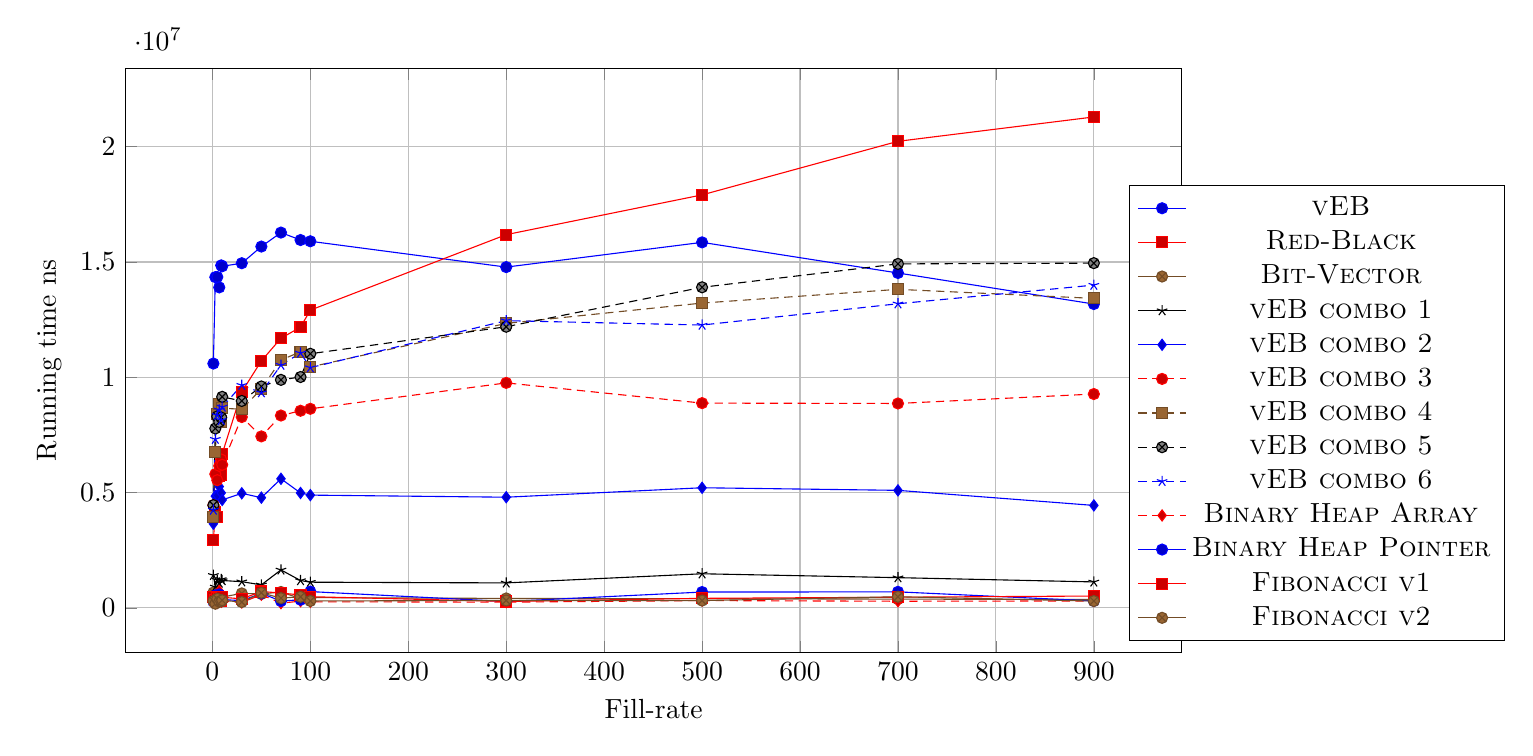
\begin{tikzpicture}
        \begin{axis}[
            xlabel = Fill-rate,
            ylabel = Running time ns,
            height=9cm,
            width=15cm,
            grid=major,
            legend style={
            at={(0.95,0.8)},
            anchor=north west}]            
            legend pos=center west
    	]
    		
    		
    	\addplot coordinates {
(1,10594290)
(3,14341481)
(5,14347849)
(7,13897463)
(9,14851770)
(10,14813042)
(30,14945554)
(50,15667620)
(70,16274540)
(90,15951603)
(100,15897028)
(300,14777090)
(500,15849857)
(700,14521126)
(900,13174934)

    	};
        
    	\addlegendentry{\textsc{vEB}}

                \addplot coordinates {
(1,2946080)
(3,4139732)
(5,3935356)
(7,5721888)
(9,5744907)
(10,6677458)
(30,9366338)
(50,10708854)
(70,11691602)
(90,12172518)
(100,12910732)
(300,16184309)
(500,17909156)
(700,20232455)
(900,21289179)

    	};
        
    	\addlegendentry{\textsc{Red-Black}}

        \addplot coordinates {
(1,662805)
(3,439108)
(5,410337)
(7,424816)
(9,415643)
(10,466015)
(30,625763)
(50,601039)
(70,688058)
(90,400927)
(100,442912)
(300,407291)
(500,395255)
(700,377521)
(900,362217)

    	};
        
    	\addlegendentry{\textsc{Bit-Vector}}

        \addplot coordinates {
(1,1411611)
(3,903893)
(5,1197517)
(7,1075567)
(9,1231658)
(10,1185278)
(30,1132512)
(50,996593)
(70,1643994)
(90,1184076)
(100,1111891)
(300,1080472)
(500,1476362)
(700,1308084)
(900,1123248)

    	};
        
    	\addlegendentry{\textsc{vEB combo 1}}

        \addplot coordinates {
(1,3646405)
(3,4842905)
(5,4875403)
(7,5257376)
(9,4985112)
(10,4680443)
(30,4965873)
(50,4776142)
(70,5596808)
(90,4981562)
(100,4888138)
(300,4797253)
(500,5207163)
(700,5094975)
(900,4441310)

    	};
        
    	\addlegendentry{\textsc{vEB combo 2}}

        \addplot coordinates {
(1,4453055)
(3,5800057)
(5,5536270)
(7,6156904)
(9,6433462)
(10,6203890)
(30,8274155)
(50,7435298)
(70,8339659)
(90,8546644)
(100,8631109)
(300,9755207)
(500,8877829)
(700,8862837)
(900,9271803)

    	};
        
    	\addlegendentry{\textsc{vEB combo 3}}
		
        \addplot coordinates {
(1,3929928)
(3,6763380)
(5,8406370)
(7,8853837)
(9,8078463)
(10,8658029)
(30,8611522)
(50,9496998)
(70,10743365)
(90,11106502)
(100,10445735)
(300,12335605)
(500,13217234)
(700,13812615)
(900,13420244)

    	};
        
    	\addlegendentry{\textsc{vEB combo 4}}
		
        \addplot coordinates {
(1,4453544)
(3,7778047)
(5,8301902)
(7,8062266)
(9,8256673)
(10,9150457)
(30,8971717)
(50,9600746)
(70,9886461)
(90,10009940)
(100,11019309)
(300,12190062)
(500,13901319)
(700,14916431)
(900,14949103)

    	};
        
    	\addlegendentry{\textsc{vEB combo 5}}

        \addplot coordinates {
(1,4241723)
(3,7313558)
(5,8351169)
(7,8584518)
(9,8136607)
(10,8711475)
(30,9654431)
(50,9331158)
(70,10527132)
(90,11051669)
(100,10416557)
(300,12454464)
(500,12264743)
(700,13187775)
(900,13995990)

    	};
        
    	\addlegendentry{\textsc{vEB combo 6}}
		
        \addplot coordinates {
(1,321315)
(3,292556)
(5,215121)
(7,730467)
(9,262790)
(10,293748)
(30,231534)
(50,568553)
(70,202894)
(90,289182)
(100,261174)
(300,246311)
(500,313787)
(700,286012)
(900,298242)

    	};
        
    	\addlegendentry{\textsc{Binary Heap Array}}

        \addplot coordinates {
(1,267939)
(3,541067)
(5,280841)
(7,578232)
(9,351427)
(10,357939)
(30,311950)
(50,625101)
(70,294468)
(90,349736)
(100,703284)
(300,273574)
(500,683813)
(700,692211)
(900,298164)

    	};
        
    	\addlegendentry{\textsc{Binary Heap Pointer}}

        \addplot coordinates {
(1,456146)
(3,337502)
(5,444872)
(7,446978)
(9,319553)
(10,457759)
(30,388491)
(50,707796)
(70,640301)
(90,558117)
(100,482365)
(300,276934)
(500,410785)
(700,460260)
(900,511763)

    	};
        
    	\addlegendentry{\textsc{Fibonacci v1}}

        \addplot coordinates {
(1,294266)
(3,177667)
(5,393286)
(7,268096)
(9,281338)
(10,328198)
(30,249705)
(50,649602)
(70,420986)
(90,477994)
(100,297104)
(300,318921)
(500,313547)
(700,479806)
(900,293045)

    	};
        
    	\addlegendentry{\textsc{Fibonacci v2}}

        \end{axis}

    \end{tikzpicture}
    \captionof{figure}{TITEL}
    \label{fig:sample_figure}
\end{minipage}

The four heaps are staying at the bottom and the Red-Black tree again shows that it behaves the wors for large fill-rates. Interestingly, both the Bit-Vector and the 1-layer van Emde Boas has almost the same running times. Each additional layer of van Emde Boas almost has the same difference between them.

\subsection{Results for testing $\FindMin$}

In this test we fill the data-structures with data and then try to find the minimum element EPP times. This should not be unfair to Fibonacci v2 since the test is constructed such that the entire data-structure has no remaining work.

\begin{minipage}[c]{\textwidth}
\advance\leftskip-2.5cm
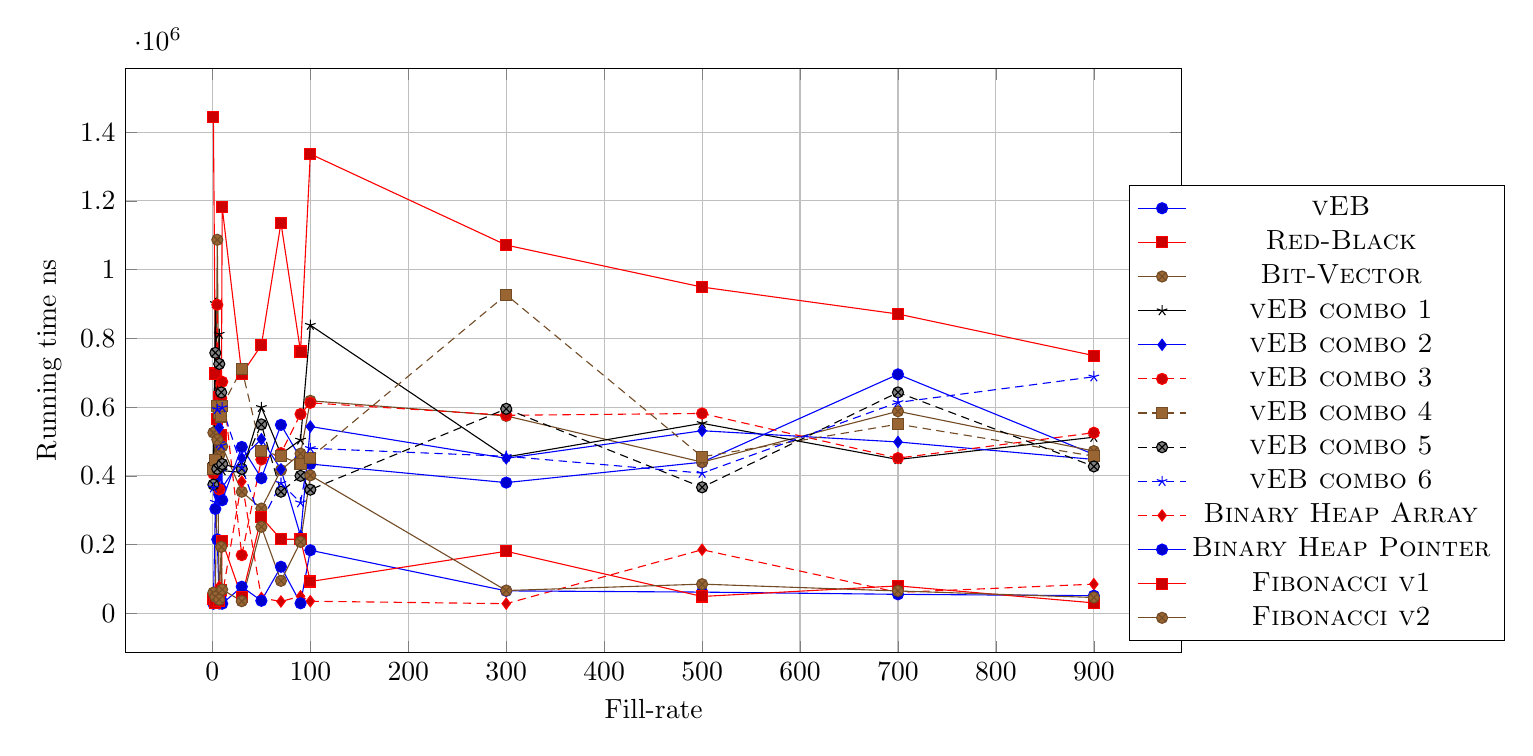
\begin{tikzpicture}
        \begin{axis}[
            xlabel = Fill-rate,
            ylabel = Running time ns,
            height=9cm,
            width=15cm,
            grid=major,
            legend style={
            at={(0.95,0.8)},
            anchor=north west}]            
            legend pos=center west
    	]
    		
    		
    	\addplot coordinates {
(1,411467)
(3,419907)
(5,418990)
(7,345191)
(9,426893)
(10,329012)
(30,484078)
(50,393117)
(70,548259)
(90,451322)
(100,434279)
(300,380261)
(500,439671)
(700,695233)
(900,462282)

    	};
        
    	\addlegendentry{\textsc{vEB}}

                \addplot coordinates {
(1,1444271)
(3,697573)
(5,565651)
(7,627716)
(9,517436)
(10,1181795)
(30,696178)
(50,780062)
(70,1135701)
(90,761678)
(100,1336519)
(300,1071411)
(500,949254)
(700,870840)
(900,749795)

    	};
        
    	\addlegendentry{\textsc{Red-Black}}

        \addplot coordinates {
(1,525641)
(3,429699)
(5,1086857)
(7,459766)
(9,485019)
(10,485650)
(30,353656)
(50,304776)
(70,416690)
(90,464637)
(100,618374)
(300,574331)
(500,439896)
(700,587783)
(900,472059)

    	};
        
    	\addlegendentry{\textsc{Bit-Vector}}

        \addplot coordinates {
(1,434133)
(3,901876)
(5,612788)
(7,812396)
(9,441655)
(10,415051)
(30,410095)
(50,599370)
(70,463216)
(90,504442)
(100,838419)
(300,454945)
(500,552772)
(700,447540)
(900,512355)

    	};
        
    	\addlegendentry{\textsc{vEB combo 1}}

        \addplot coordinates {
(1,418044)
(3,436778)
(5,392901)
(7,540316)
(9,629476)
(10,365446)
(30,451527)
(50,506639)
(70,419024)
(90,225327)
(100,543484)
(300,451017)
(500,531224)
(700,498564)
(900,447644)

    	};
        
    	\addlegendentry{\textsc{vEB combo 2}}

        \addplot coordinates {
(1,406402)
(3,417654)
(5,897772)
(7,360605)
(9,625768)
(10,673639)
(30,169161)
(50,447536)
(70,466042)
(90,579751)
(100,612423)
(300,576195)
(500,581470)
(700,451537)
(900,525479)

    	};
        
    	\addlegendentry{\textsc{vEB combo 3}}
		
        \addplot coordinates {
(1,419638)
(3,447134)
(5,602287)
(7,583223)
(9,572636)
(10,602073)
(30,711592)
(50,473060)
(70,456780)
(90,434763)
(100,452977)
(300,926780)
(500,455383)
(700,550311)
(900,457234)

    	};
        
    	\addlegendentry{\textsc{vEB combo 4}}
		
        \addplot coordinates {
(1,374544)
(3,757789)
(5,420380)
(7,725510)
(9,642733)
(10,434190)
(30,420070)
(50,549607)
(70,353724)
(90,399984)
(100,359688)
(300,594955)
(500,366602)
(700,642710)
(900,427314)

    	};
        
    	\addlegendentry{\textsc{vEB combo 5}}

        \addplot coordinates {
(1,365157)
(3,323496)
(5,593226)
(7,494380)
(9,488078)
(10,598580)
(30,425125)
(50,265587)
(70,378567)
(90,322002)
(100,480102)
(300,456905)
(500,407874)
(700,613610)
(900,688276)

    	};
        
    	\addlegendentry{\textsc{vEB combo 6}}
		
        \addplot coordinates {
(1,47109)
(3,57735)
(5,55106)
(7,77634)
(9,37275)
(10,50996)
(30,383042)
(50,44659)
(70,34304)
(90,49530)
(100,35064)
(300,28019)
(500,185021)
(700,60811)
(900,84797)

    	};
        
    	\addlegendentry{\textsc{Binary Heap Array}}

        \addplot coordinates {
(1,27910)
(3,303825)
(5,214904)
(7,28504)
(9,38125)
(10,27837)
(30,77383)
(50,36402)
(70,135356)
(90,29125)
(100,183360)
(300,65257)
(500,61646)
(700,55192)
(900,51200)

    	};
        
    	\addlegendentry{\textsc{Binary Heap Pointer}}

        \addplot coordinates {
(1,41858)
(3,29639)
(5,52048)
(7,36365)
(9,68282)
(10,210583)
(30,46546)
(50,279261)
(70,215478)
(90,215615)
(100,92468)
(300,180415)
(500,48989)
(700,79695)
(900,30252)

    	};
        
    	\addlegendentry{\textsc{Fibonacci v1}}

        \addplot coordinates {
(1,60214)
(3,47779)
(5,505466)
(7,39654)
(9,193198)
(10,68973)
(30,35198)
(50,251651)
(70,94384)
(90,207580)
(100,401449)
(300,66212)
(500,84847)
(700,64945)
(900,46023)

    	};
        
    	\addlegendentry{\textsc{Fibonacci v2}}

        \end{axis}

    \end{tikzpicture}
    \captionof{figure}{Time of $\FindMin$ for fill-rates 1 to 900}
    \label{fig:sample_figure}
\end{minipage}


The results are a bit more spread out this time and there are of odd points from 0 to 100 in fill-rate. However, one should notice that the tics on the y-axis is 200 microseconds, so a context-switch can have a lot of impact. We see the Red-Black tree perform the worst, which makes sense since it has no constant time lookup for $\Minimum$. The Bit-Vectors and van Emde Boas Trees are placed nicely int he middle and then we have the heaps at the bottom.

\section{Summary on priority queues vs search trees results}

We must admit we were rather suprised by the outcome of the tests. We had anticipated that the search trees perform much worse than they had and the only test we thought it would tie, $\FindMin$ it wound up loosing. The performance of the van Emde Boas Tree with two layers and then Bit-Vectors seems as a fair compromise if one would not put in the effort to build a heap.


\chapter{Arithmetic operations}

Everytime we recurse in our van Emde Boas trees we perform the same arithmetic operations to figure out where to divide the bits in an upper and lower half. As a result of the combo tree implementation, it was more natural to keep the universe in size of bits than having the universe in integer representation. 

This lead us to investigate if there was a difference in how the computer calculated the operations. Corman et al writes in their implementation that higher can be found as $\HIGHER = 2^{\lceil{(\log u)/2}\rceil}$. A naive implementation might be something like:
\begin{lstlisting}
pow(2, (int)ceil((log2 (u))/2));
\end{lstlisting}

So this would make a few different calls to the math package being log2, ceil and power. log2 can be found by MSB which we have seen a constant time operation for, but we are trying to bring down the number of instructions and measure the total time. There is also a cast in there. It would be fun to see if we could do it faster. All tests has been run with a Clang compiler with 3rd level of optimization, so we do not expect to get results that are much higher . This is the different ways we calculate $\HIGHER$:

\begin{lstlisting}
1: pow(2, (int)ceil((log2 (u))/2));

2: result = 1<<(int)ceil((log2 (u))/2);

3: uint32_t b = log2 (u);
   uint32_t h = (b >> 1) + (b & 1);
   result = 1<<h;

4: result = 1<<(int)ceil((log2_x86 (u))/2);

5: uint32_t b = log2_x86 (u);
   uint32_t h = (b >> 1) + (b & 1);
   result = 1<<h;

6: uint32_t b = log2_table (u);
   uint32_t h = (b >> 1) + (b & 1);
   result = 1<<h;

\end{lstlisting}

log2\_x86 is just the MSB instruction that can be found on x86 architectures with the assembly instruction bsr. log2\_table is a computed table that gives the result by a lookup. We are performing 100.000 calculations and then divide the total time by the same amount. We have compiled all the tests the Clang compiler without any optimizations and the Clang compiler with the most aggresive optimatization. We will use 1 as the measurement for how well the other test performs:

\begin{center}
  \begin{tabular}{ l | c | c | c | c }
    Method & Clang no opt & Clang with opt & \% faster no opt & \% faster opt  \\ \hline
    1 & 288 & 185 & 0 & 0 \\ 
    2 & 179 & 171 & 38 & 8\\ 
    3 & 178 & 170 & 38 & 8 \\ 
    4 & 173 & 163 & 40 & 12\\ 
    4 & 174 & 161 & 40 & 13 \\ 
    6 & 182 & 164 & 37 & 11 \\ 
  \end{tabular}
\end{center}

We must assume that the most people would compile their van Emde Boas trees with optimization turned on, if not, a better arithmetic approach could yield a 40 \% quicker tree. But still, if optimization is turned on, the crucial arithmetic used for seperating bits can still be made 13 \% quicker.

\chapter{Conlusion}

We have shown a total of 9 different data-structures that each perform the duties described by a search tree. We have shown that the best candidate when considering run times is a combo tree with two layers of van Emde Boas trees and a bit-vector of size 64????? at every leaf.

We also showed that the search structures all performs worse than our heap implementations from a previous project, however, the combo tree with 2 layers performs the best of the trees and is very close to the binary heap with pointers.

When running our tests on the data structures we took interest in how to find the top and the bottom part of the bits effectively. We showed that the calculation for upper could be done 40 \% faster if no optimization was used when compiling and 13 \% faster with optimization being turned on compared to a straight forward naive approach. 


%%%%%%%%%%%%%%%%%%%%%%%%%%%%%%%%%%%%%%%%%%%%%%%%%%%%%%%%%%%%%%%%%%%%%%%

\addcontentsline{toc}{chapter}{Bibliography}
\bibliographystyle{plain} 
\bibliography{report}

\end{document}

